%%%%%   Capitulo 4 : Diseño Basico    %%%%%
\chapter{Diseño Básico}

\section{Metología del Diseño Básico}
Posterior a la fase de diseño conceptual de la solución, se presenta el diseño básico del mismo, en donde se divide el dispositivo en una serie de subsistemas. Esto con el propósito facilitar el entendimiento de los principios físicos que describen el comportamiento de las diferentes partes del equipo, así como las teorías de diseño empleadas para el dimensionamiento de sus partes. De estas teorías se destacan las de diseño mecánico, las cuales permite el dimensionamiento de un elemento sometido a una condición de esfuerzos, dada una geometría, como son las teorías de fallas para materiales dúctiles (Esfuerzo cortante máximo, Energía de distorsión y Mohr Coulomb dúctil) y para materiales frágiles (Esfuerzo normal máximo, Mohr Coulomb frágil y Mohr modificada) \citep{shigley2011shigley}.

Para este proyecto, la máquina a diseñar se dividió en 6 apartados (también ver Figura \ref{fig:subsystems}):

\begin{itemize} \nosep
    \item El Husillo, es el sistema de accionamiento de la herramienta de corte.
    \item El Mecanismo, es el sistema que transmite el movimiento de los actuadores a la herramienta de corte.
    \item El Accionamiento, es el sistema de actuación que convierten la energía primaria en energía mecánica.
    \item La Estructura, es el sistema que brinda el soporte y el cual sostiene todos los demás subsistemas.
    \item El Sistema de Control, es el sistema que manipula el sistema de accionamiento para posicionar la herramienta durante el corte.
    \item El Sistema de Refrigeración, es el sistema que mantiene la temperatura, tanto de la pieza como la de herramienta, en valores aceptables para el proceso.
\end{itemize}

El alcance del proyecto llegará hasta el diseño básico de la estructura, dejando para próximos proyectos y/o trabajos el diseño de las demás subsistemas de esta máquina. En las siguientes secciones de este capítulo se desarrollará el diseño de cada apartado.

\begin{figure}[ht!]
    \centering
    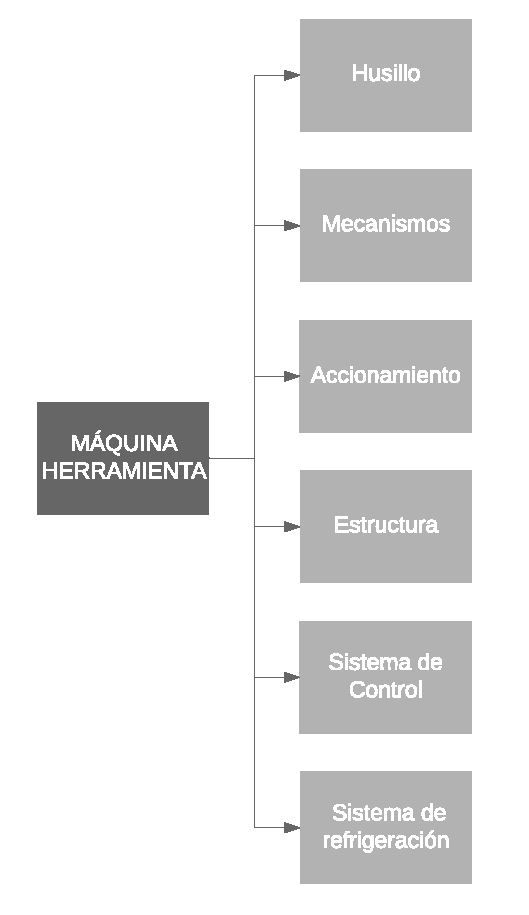
\includegraphics[height = 0.7\textheight]{Cap4_DisenoBasico/Figura/Subsistemas.pdf}
    \caption{Subsistemas presentes en la máquina}
    \label{fig:subsystems}
\end{figure}
\newpage

%%%%%   Diseño Basico Husillo    %%%%%
\section{Diseño Básico del Husillo}
Para el básico del sistema de corte motor-husillo se toma como guía los catálogos de herramientas de corte  \cite{catalogue:CatalogoC006s} y \cite{catalogue:Blue_Master} , para asi obtener los parámetros corte y variables a considerar para el cálculo de potencia de corte ($P_c$). 

\subsection{Parámetros de corte recomendados para fresas HSS-Co8}

En el dimensionamiento del motor-husillo se utilizaron parámetros de corte recomendados por el fabrícate de fresas \cite{catalogue:Blue_Master} donde especifica las velocidades de corte ($V_C$) y velocidades de avance($V_f$) dependiendo del material del que está hecha la pieza de trabajo y las características de la herramienta de corte fresa. En este mismo catalogo también recomiendo ancho de corte($e_p$) y profundidad de corte ($a_p$), los cuales depende del diámetro de la herramienta de corte y el tipo de operación.. Los diámetros con lo que se quiere trabajar en las operaciones de fresado esta entre 2 a 18 mm y los materiales de las piezas a trabajar serán aluminio y acero blando. Los parámetros se presentaron en la tabla \ref{table:Parametro_de_corte}.\\


% Please add the following required packages to your document preamble:
% \usepackage{multirow}
% \usepackage[table,xcdraw]{xcolor}
% If you use beamer only pass "xcolor=table" option, i.e. \documentclass[xcolor=table]{beamer}
\begin{longtable}{|c|c|c|c|c|c|c|c|}\hline
\rowcolor[HTML]{EFEFEF} 
\multicolumn{3}{|c|}{\cellcolor[HTML]{EFEFEF}} & \multicolumn{5}{c|}{\cellcolor[HTML]{EFEFEF}Diametro (mm)} \\ \cline{4-8} 
\rowcolor[HTML]{EFEFEF} 
\multicolumn{3}{|c|}{\multirow{-2}{*}{\cellcolor[HTML]{EFEFEF}}}                                                                                                                                                                                    & 2   & 4  & 8  & 10& 18\\ \hline
\rowcolor[HTML]{EFEFEF} 
\cellcolor[HTML]{EFEFEF}  & \begin{tabular}[c]{@{}c@{}}Velocidad de \\ corte (m / min)\end{tabular}  & \cellcolor[HTML]{EFEFEF}  & \multicolumn{5}{c|}{\cellcolor[HTML]{EFEFEF}Velocidad angular(RPM)} \\ \cline{2-2} \cline{4-8} 
\rowcolor[HTML]{EFEFEF} 
\cellcolor[HTML]{EFEFEF}                                                                                                                                       & 39                                                                                        & \multirow{-2}{*}{\cellcolor[HTML]{EFEFEF}N ° de filos} & 6207         & 3104         & 1552        & 1241        & 690       \\ \cline{2-8} 
\cellcolor[HTML]{EFEFEF}                                                                                                                                       &                                                                                           & 2                                                      & 50           & 56           & 84          & 82          & 80        \\ \cline{3-8} 
\cellcolor[HTML]{EFEFEF}                                                                                                                                       &                                                                                           & 3                                                      & 75           & 84           & 126         & 123         & 120       \\ \cline{3-8} 
\multirow{-5}{*}{\cellcolor[HTML]{EFEFEF}\begin{tabular}[c]{@{}c@{}}Acero blando \\ \\ Resistencia a la tracción \\  70 Kg / mm \textasciicircum 2\end{tabular}} & \multirow{-3}{*}{\begin{tabular}[c]{@{}c@{}}Velocidad de \\ avance (mm/min)\end{tabular}} & 4                                                      & 100          & 112          & 168         & 164         & 160       \\ \hline
\rowcolor[HTML]{EFEFEF} 
\cellcolor[HTML]{EFEFEF}                                                                                                                                       & \begin{tabular}[c]{@{}c@{}}Velocidad de \\ corte (m / min)\end{tabular}                   & \cellcolor[HTML]{EFEFEF}                               & \multicolumn{5}{c|}{\cellcolor[HTML]{EFEFEF}Velocidad angular(RPM)} \\ \cline{2-2} \cline{4-8} 
\rowcolor[HTML]{EFEFEF} 
\cellcolor[HTML]{EFEFEF}                                                                                                                                       & 230                                                                                       & \multirow{-2}{*}{\cellcolor[HTML]{EFEFEF}N ° de filos} & 36606        & 18303        & 9152        & 7321        & 4067      \\ \cline{2-8} 
\cellcolor[HTML]{EFEFEF}                                                                                                                                       &                                                                                           & 2                                                      & 293          & 329          & 494         & 400         & 230       \\ \cline{3-8} 
\cellcolor[HTML]{EFEFEF}                                                                                                                                       &                                                                                           & 3                                                      & 440          & 494          & 741         & 600         & 345       \\ \cline{3-8} 
\multirow{-5}{*}{\cellcolor[HTML]{EFEFEF}Aluminio}                                                                                                             & \multirow{-3}{*}{\begin{tabular}[c]{@{}c@{}}Velocidad de \\ avance (mm/min)\end{tabular}} & 4                                                      & 586          & 658          & 988         & 800         & 460       \\ \hline
\caption{Parametros de corte para el Acero blando y aluminio}{Fuente:\citep{catalogue:Blue_Master}}
\label{table:Parametro_de_corte}
\end{longtable}

En la Figura \ref{fig:Profun} se presenta las profundidades recomendadas para tres distintas operaciones.  

\begin{figure}[hbt]
    \centering
    \begin{subfigure}{0.3\textwidth}
        \centering
        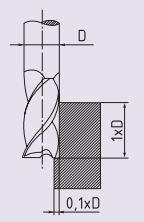
\includegraphics[width=0.9\linewidth]{Cap4_DisenoBasico/Figura/Fresado_Lateral.PNG}
        \caption{Fresado Lateral}
        \label{fig:Fresado_Lateral}
    \end{subfigure} 
    \centering
    \begin{subfigure}{0.3\textwidth}
        \centering
        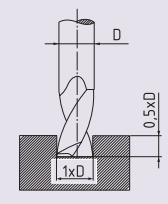
\includegraphics[width=0.9\linewidth]{Cap4_DisenoBasico/Figura/Ranurado.PNG}
        \caption{Vaciado}
        \label{fig:VAciado}
    \end{subfigure} 
    \centering
    \begin{subfigure}{0.3\textwidth}
        \centering
        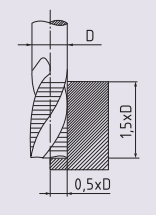
\includegraphics[width=0.9\linewidth]{Cap4_DisenoBasico/Figura/Basto.PNG}
        \caption{Basto}
        \label{fig:Basto}
    \end{subfigure} 
    \caption{Profucidad y ancho de corte recomendada del fresado}{Fuente: \citep{catalogue:Blue_Master}}
    \label{fig:Profun}
\end{figure}

Para preservar la vida útil de herramienta de corte y tener un menor consumo de potencia se plantea que para el aluminio en el fresado Basto la profundidad corte ($a_p$) a partir del diámetro de 8 mm en adelante será de 10 $mm$ y para el fresado ranurado o vaciado la profundidad es $0.3$ el diametro de la fresa. De igual forma para el acero blando se toma tambien una progundidad de corte similar a la de fresado basto pero el ancho de corte será $0.25$ el diametro de la herramienta, y en el ranurado la profundidad de corte será $0.2$ el diametro de la herramineta de fresado. En la tabla \ref{table:Profundidad_aluminio} y la tabla \ref{table:Profundidad_acero} se presentará el ancho y profundidad de corte para los tipos de fresado .

Con los parámetros ya obtenidos, se procede a usar la expresión encontrada en catálogo de \cite{catalogue:CatalogoC006s} donde,  relacionan los parámetros de corte con un término llamado presión especifica de corte que esta tabulada con respecto al avance por diente. La ecuacion \ref{Eq:P_c} es la expresión para el calculo de la potencia de corte.

% Please add the following required packages to your document preamble:
% \usepackage[table,xcdraw]{xcolor}
% If you use beamer only pass "xcolor=table" option, i.e. \documentclass[xcolor=table]{beamer}

\begin{longtable}{|>{\columncolor[HTML]{EFEFEF}}c |c|c|c|c|c|c|}
\hline
\multicolumn{2}{|c|}{\cellcolor[HTML]{EFEFEF}Diametro ($mm$)}                  & \multicolumn{1}{l|}{\cellcolor[HTML]{EFEFEF}2} & \multicolumn{1}{l|}{\cellcolor[HTML]{EFEFEF}4} & \multicolumn{1}{l|}{\cellcolor[HTML]{EFEFEF}8} & \multicolumn{1}{l|}{\cellcolor[HTML]{EFEFEF}10} & \multicolumn{1}{l|}{\cellcolor[HTML]{EFEFEF}18} \\ \hline
\multicolumn{7}{|c|}{\cellcolor[HTML]{EFEFEF}Fresado Lateral}   \\ \hline
\begin{tabular}[c]{@{}c@{}}Profundidad\\   de corte (mm)\end{tabular} & ap & 2& 4 & 8& 10& 18\\ \hline
\begin{tabular}[c]{@{}c@{}}Ancho de\\   corte (mm)\end{tabular}       & ep & 0,2& 0,4 & 0,8& 1& 1,8\\ \hline
\multicolumn{7}{|c|}{\cellcolor[HTML]{EFEFEF}Vaciado} \\ \hline
\begin{tabular}[c]{@{}c@{}}Profundidad\\   de corte(mm)\end{tabular}  & ap & 0,6 & 1,2 & 2,4 & 3 & 5,4\\ \hline
\begin{tabular}[c]{@{}c@{}}Ancho de\\   corte(mm)\end{tabular}        & ep & 2 & 4 & 8 & 10 & 18 \\ \hline
\multicolumn{7}{|c|}{\cellcolor[HTML]{EFEFEF}Basto}\\ \hline
\begin{tabular}[c]{@{}c@{}}Profundidad\\   de corte(mm)\end{tabular}  & ap & 3& 6& 10 & 10 & 10\\ \hline
\begin{tabular}[c]{@{}c@{}}Ancho de\\   corte(mm)\end{tabular} & ep & 1  & 2 & 4 & 5 & 9  \\ \hline

\caption{Profundidad y ancho de corte para aluminio}{Fuente:\cite{catalogue:Blue_Master}}
\label{table:Profundidad_aluminio}
\end{longtable}



% Please add the following required packages to your document preamble:
% \usepackage[table,xcdraw]{xcolor}
% If you use beamer only pass "xcolor=table" option, i.e. \documentclass[xcolor=table]{beamer}

\begin{longtable}{|>{\columncolor[HTML]{EFEFEF}}c |c|c|c|c|c|c|}
\hline
\hline
\multicolumn{2}{|c|}{\cellcolor[HTML]{EFEFEF}Diametro ($mm$)} & \multicolumn{1}{l|}{\cellcolor[HTML]{EFEFEF}2} & \multicolumn{1}{l|}{\cellcolor[HTML]{EFEFEF}4} & \multicolumn{1}{l|}{\cellcolor[HTML]{EFEFEF}8} & \multicolumn{1}{l|}{\cellcolor[HTML]{EFEFEF}10} & \multicolumn{1}{l|}{\cellcolor[HTML]{EFEFEF}18} \\ \hline
\multicolumn{7}{|c|}{\cellcolor[HTML]{EFEFEF}Fresado Lateral}\\ \hline
\begin{tabular}[c]{@{}c@{}}Profundidad\\   de corte (mm)\end{tabular} & ap & 2& 4 & 8& 10& 18\\ \hline
\begin{tabular}[c]{@{}c@{}}Ancho de\\   corte (mm)\end{tabular}       & ep & 0,2& 0,4 & 0,8& 1& 1,8\\ \hline
\multicolumn{7}{|c|}{\cellcolor[HTML]{EFEFEF}Vaciado} \\ \hline
\begin{tabular}[c]{@{}c@{}}Profundidad\\   de corte(mm)\end{tabular}  & ap & 0.4 & .8 & 1.6 & 2 & 3.6\\ \hline
\begin{tabular}[c]{@{}c@{}}Ancho de\\   corte(mm)\end{tabular}        & ep & 2 & 4 & 8 & 10 & 18 \\ \hline
\multicolumn{7}{|c|}{\cellcolor[HTML]{EFEFEF}Basto}\\ \hline
\begin{tabular}[c]{@{}c@{}}Profundidad\\   de corte(mm)\end{tabular}  & ap & 3& 6& 10 & 10 & 10\\ \hline
\begin{tabular}[c]{@{}c@{}}Ancho de\\   corte(mm)\end{tabular} & ep & 0.5  & 1 & 2 & 2.5 & 4.5  \\ \hline

\caption{Profundidad y ancho de corte para acero}{Fuente:\cite{catalogue:Blue_Master}}
\label{table:Profundidad_acero}
\end{longtable}
\begin{equation}
    P_{c}=\frac{a_{p}*a_{e}*f_{r}*K_{c}}{60*10^6*\eta}
    \label{Eq:P_c}
\end{equation}
Donde $a_{e}$ es el ancho de corte en ($mm$), $a_{p}$ es la profundidad de corte en $mm$, $f_{r}$ es la velocidad de avance en ($mm/min$), $\eta $ es la eficiencia de la operación que depende del desgate de la herramienta y de la máquina, y $K_{c}$ es  la presión especifica  de corte que depende del materia y de la carga de viruta $f$.

\newpage
\subsection{Potencias y Pares requeridos para fresado.}

En catalogo \cite{catalogue:CatalogoC006s} existe la tabla la cual relaciona la el avance por diente o la carga de viruta con la presión especifica $K_{c}$ de distintos materiales como acero dulce, acero para herramientas, titanio y aluminios. Se tomará la presión especifica de corte con la carga de viruta de 0.1$mm/diente$ ya que este da el mayor valor de este parámetro para cada material. Los materiales que se tomaron para el cálculo fueron una aleación ligera de aluminio (Al-Zn-Mg-Cu) y un acero con una resistencia a la tracción similar a la del catálogo \cite{catalogue:Blue_Master} el cual fua un acero para herramientas con una resistencia a la tracción de 670 $Mpa$. En la tabla \ref{table:K_C} se muesta los valores de la la presion especifica de corte.
\begin{longtable}{|
>{\columncolor[HTML]{EFEFEF}}c |c|c|}
\hline
\cellcolor[HTML]{EFEFEF}                          & \cellcolor[HTML]{EFEFEF}                                                                                               & \cellcolor[HTML]{EFEFEF}\begin{tabular}[c]{@{}c@{}}Presion de corte especifica\\     (Mpa)\end{tabular} \\\cline{3-3} 
\multirow{-2}{*}{\cellcolor[HTML]{EFEFEF}Materia} & \multirow{-2}{*}{\cellcolor[HTML]{EFEFEF}\begin{tabular}[c]{@{}c@{}}Resistecia a la tracción\\ (Mpa)\end{tabular}} & \cellcolor[HTML]{EFEFEF}0.1 mm/diente \\ \hline
Acero para Herramientas & 670& 1980\\ \hline
Aleacion ligera (Al-Zn-Mg-Cu) & 570& 880 \\ \hline
\caption{Presion de corte especifica}{Fuente:\citep{catalogue:CatalogoC006s}}
\label{table:K_C}
\end{longtable}

%table:Potencia_de_corte_A
Las potencias de actuales para el fresado del aluminio y el acero blando se calcularon con la ecuación \ref{Eq:P_c} y presentan en las tablas \ref{table:Potencia_de_corte_A} y \ref{table:Potencia_de_corte_Acero} respectivamente. Con los resultados de las potencias se busca los pares máximos que requiere para los distintos materiales (aluminio, acero) con la ecuación \ref{Eq:T_{r}}. 

%longtable

\begin{longtable}{|l|
>{\columncolor[HTML]{EFEFEF}}c |
>{\columncolor[HTML]{EFEFEF}}c |
>{\columncolor[HTML]{EFEFEF}}c |
>{\columncolor[HTML]{EFEFEF}}c |
>{\columncolor[HTML]{EFEFEF}}c |
>{\columncolor[HTML]{EFEFEF}}c |
>{\columncolor[HTML]{EFEFEF}}c |
>{\columncolor[HTML]{EFEFEF}}c |
>{\columncolor[HTML]{EFEFEF}}c |
>{\columncolor[HTML]{EFEFEF}}c |
>{\columncolor[HTML]{EFEFEF}}c |
>{\columncolor[HTML]{EFEFEF}}c |
>{\columncolor[HTML]{EFEFEF}}c |
>{\columncolor[HTML]{EFEFEF}}c |
>{\columncolor[HTML]{EFEFEF}}c |}
\hline
\cellcolor[HTML]{EFEFEF}                                & \multicolumn{15}{c|}{\cellcolor[HTML]{EFEFEF}Aluminio}                                                                                                                                                                                                                                                                                                                                                                                                                                                                                                                                                                                                                                                                                                             \\ \cline{2-16} 
\cellcolor[HTML]{EFEFEF}                                & \multicolumn{5}{c|}{\cellcolor[HTML]{EFEFEF}\begin{tabular}[c]{@{}c@{}}Potencia actuar \\ Fresado Lateral (Kw)\end{tabular}}                                                                                                                         & \multicolumn{5}{c|}{\cellcolor[HTML]{EFEFEF}\begin{tabular}[c]{@{}c@{}}Potencia actuar \\ Fresado Ranurado (Kw)\end{tabular}}                                                                                                                        & \multicolumn{5}{c|}{\cellcolor[HTML]{EFEFEF}\begin{tabular}[c]{@{}c@{}}Potencia actuar \\ Fresado Basto(Kw)\end{tabular}} \\ \cline{2-16} 
\cellcolor[HTML]{EFEFEF}                                & \multicolumn{15}{c|}{\cellcolor[HTML]{EFEFEF}Diametro (mm)} \\ \cline{2-16} 
\multirow{-4}{*}{\cellcolor[HTML]{EFEFEF}\begin{tabular}[c]{@{}l@{}}N° de \\ dientes\end{tabular}}& \multicolumn{1}{l|}{\cellcolor[HTML]{EFEFEF}2} & \multicolumn{1}{l|}{\cellcolor[HTML]{EFEFEF}4} & \multicolumn{1}{l|}{\cellcolor[HTML]{EFEFEF}8} & \multicolumn{1}{l|}{\cellcolor[HTML]{EFEFEF}10} & \multicolumn{1}{l|}{\cellcolor[HTML]{EFEFEF}18} & \multicolumn{1}{l|}{\cellcolor[HTML]{EFEFEF}2} & \multicolumn{1}{l|}{\cellcolor[HTML]{EFEFEF}4} & \multicolumn{1}{l|}{\cellcolor[HTML]{EFEFEF}8} & \multicolumn{1}{l|}{\cellcolor[HTML]{EFEFEF}10} & \multicolumn{1}{l|}{\cellcolor[HTML]{EFEFEF}18} & \multicolumn{1}{l|}{\cellcolor[HTML]{EFEFEF}2} & \multicolumn{1}{l|}{\cellcolor[HTML]{EFEFEF}4} & \multicolumn{1}{l|}{\cellcolor[HTML]{EFEFEF}8} & \multicolumn{1}{l|}{\cellcolor[HTML]{EFEFEF}10} & \multicolumn{1}{l|}{\cellcolor[HTML]{EFEFEF}18} \\ \hline
2                                                       & \cellcolor[HTML]{FFFFFF}0,0                    & \cellcolor[HTML]{FFFFFF}0,0                    & \cellcolor[HTML]{FFFFFF}0,1                    & \cellcolor[HTML]{FFFFFF}0,1                     & \cellcolor[HTML]{FFFFFF}0,2                     & \cellcolor[HTML]{FFFFFF}0,0                    & \cellcolor[HTML]{FFFFFF}0,0                    & \cellcolor[HTML]{FFFFFF}0,2                    & \cellcolor[HTML]{FFFFFF}0,3                     & \cellcolor[HTML]{FFFFFF}0,5                     & \cellcolor[HTML]{FFFFFF}0,0                    & \cellcolor[HTML]{FFFFFF}0,1                    & \cellcolor[HTML]{FFFFFF}0,4                    & \cellcolor[HTML]{FFFFFF}0,5                     & \cellcolor[HTML]{FFFFFF}0,6                     \\ \hline
3                                                       & \cellcolor[HTML]{FFFFFF}0,0                    & \cellcolor[HTML]{FFFFFF}0,0                    & \cellcolor[HTML]{FFFFFF}0,1                    & \cellcolor[HTML]{FFFFFF}0,2                     & \cellcolor[HTML]{FFFFFF}0,3                     & \cellcolor[HTML]{FFFFFF}0,0                    & \cellcolor[HTML]{FFFFFF}0,0                    & \cellcolor[HTML]{FFFFFF}0,3                    & \cellcolor[HTML]{FFFFFF}0,5                     & \cellcolor[HTML]{FFFFFF}0,8                     & \cellcolor[HTML]{FFFFFF}0,0                    & \cellcolor[HTML]{FFFFFF}0,1                    & \cellcolor[HTML]{FFFFFF}0,6                    & \cellcolor[HTML]{FFFFFF}0,8                     & \cellcolor[HTML]{FFFFFF}0,9                     \\ \hline
4                                                       & \cellcolor[HTML]{FFFFFF}0,0                    & \cellcolor[HTML]{FFFFFF}0,0                    & \cellcolor[HTML]{FFFFFF}0,1                    & \cellcolor[HTML]{FFFFFF}0,2                     & \cellcolor[HTML]{FFFFFF}0,4                     & \cellcolor[HTML]{FFFFFF}0,0                    & \cellcolor[HTML]{FFFFFF}0,1                    & \cellcolor[HTML]{FFFFFF}0,4                    & \cellcolor[HTML]{FFFFFF}0,6                     & \cellcolor[HTML]{FFFFFF}1,0                     & \cellcolor[HTML]{FFFFFF}0,0                    & \cellcolor[HTML]{FFFFFF}0,2                    & \cellcolor[HTML]{FFFFFF}0,8                    & \cellcolor[HTML]{FFFFFF}1,0                     & \cellcolor[HTML]{FFFFFF}1,1                     \\ \hline
\caption{potencia actual aluminio}{Fuente:Elaboración propia}
\label{table:Potencia_de_corte_A}

\end{longtable} \newpage
 %longtable

\begin{longtable}{|l|
>{\columncolor[HTML]{EFEFEF}}c |
>{\columncolor[HTML]{EFEFEF}}c |
>{\columncolor[HTML]{EFEFEF}}c |
>{\columncolor[HTML]{EFEFEF}}c |
>{\columncolor[HTML]{EFEFEF}}c |
>{\columncolor[HTML]{EFEFEF}}c |
>{\columncolor[HTML]{EFEFEF}}c |
>{\columncolor[HTML]{EFEFEF}}c |
>{\columncolor[HTML]{EFEFEF}}c |
>{\columncolor[HTML]{EFEFEF}}c |
>{\columncolor[HTML]{EFEFEF}}c |
>{\columncolor[HTML]{EFEFEF}}c |
>{\columncolor[HTML]{EFEFEF}}c |
>{\columncolor[HTML]{EFEFEF}}c |
>{\columncolor[HTML]{EFEFEF}}c |} \hline
\cellcolor[HTML]{EFEFEF}                                & \multicolumn{15}{c|}{\cellcolor[HTML]{EFEFEF}Acero Blando} \\ \cline{2-16} 
\cellcolor[HTML]{EFEFEF}                                & \multicolumn{5}{c|}{\cellcolor[HTML]{EFEFEF}\begin{tabular}[c]{@{}c@{}}Potencia actuar \\ Fresado Lateral (Kw)\end{tabular}}                                                                                                                         & \multicolumn{5}{c|}{\cellcolor[HTML]{EFEFEF}\begin{tabular}[c]{@{}c@{}}Potencia actuar \\ Fresado Ranurado (Kw)\end{tabular}}                                                                                                                        & \multicolumn{5}{c|}{\cellcolor[HTML]{EFEFEF}\begin{tabular}[c]{@{}c@{}}Potencia actuar \\ Fresado Basto(Kw)\end{tabular}}                                                                                                                            \\ \cline{2-16} 
\cellcolor[HTML]{EFEFEF}                                & \multicolumn{15}{c|}{\cellcolor[HTML]{EFEFEF}Diametro (mm)}                                                                                                                                                                                                                                                                                                                                                                                                                                                                                                                                                                                                                                                                                                        \\ \cline{2-16} 
\multirow{-4}{*}{\cellcolor[HTML]{EFEFEF}\begin{tabular}[c]{@{}l@{}}N° de \\ dientes\end{tabular}} & \multicolumn{1}{l|}{\cellcolor[HTML]{EFEFEF}2} & \multicolumn{1}{l|}{\cellcolor[HTML]{EFEFEF}4} & \multicolumn{1}{l|}{\cellcolor[HTML]{EFEFEF}8} & \multicolumn{1}{l|}{\cellcolor[HTML]{EFEFEF}10} & \multicolumn{1}{l|}{\cellcolor[HTML]{EFEFEF}18} & \multicolumn{1}{l|}{\cellcolor[HTML]{EFEFEF}2} & \multicolumn{1}{l|}{\cellcolor[HTML]{EFEFEF}4} & \multicolumn{1}{l|}{\cellcolor[HTML]{EFEFEF}8} & \multicolumn{1}{l|}{\cellcolor[HTML]{EFEFEF}10} & \multicolumn{1}{l|}{\cellcolor[HTML]{EFEFEF}18} & \multicolumn{1}{l|}{\cellcolor[HTML]{EFEFEF}2} & \multicolumn{1}{l|}{\cellcolor[HTML]{EFEFEF}4} & \multicolumn{1}{l|}{\cellcolor[HTML]{EFEFEF}8} & \multicolumn{1}{l|}{\cellcolor[HTML]{EFEFEF}10} & \multicolumn{1}{l|}{\cellcolor[HTML]{EFEFEF}18} \\ \hline
2                                                       & \cellcolor[HTML]{FFFFFF}0,00                   & \cellcolor[HTML]{FFFFFF}0,00                   & \cellcolor[HTML]{FFFFFF}0,03                   & \cellcolor[HTML]{FFFFFF}0,04                    & \cellcolor[HTML]{FFFFFF}0,12                    & \cellcolor[HTML]{FFFFFF}0,00                   & \cellcolor[HTML]{FFFFFF}0,01                   & \cellcolor[HTML]{FFFFFF}0,05                   & \cellcolor[HTML]{FFFFFF}0,08                    & \cellcolor[HTML]{FFFFFF}0,24                    & \cellcolor[HTML]{FFFFFF}0,00                   & \cellcolor[HTML]{FFFFFF}0,02                   & \cellcolor[HTML]{FFFFFF}0,08                   & \cellcolor[HTML]{FFFFFF}0,10                    & \cellcolor[HTML]{FFFFFF}0,17                    \\ \hline
3                                                       & \cellcolor[HTML]{FFFFFF}0,00                   & \cellcolor[HTML]{FFFFFF}0,01                   & \cellcolor[HTML]{FFFFFF}0,04                   & \cellcolor[HTML]{FFFFFF}0,06                    & \cellcolor[HTML]{FFFFFF}0,18                    & \cellcolor[HTML]{FFFFFF}0,00                   & \cellcolor[HTML]{FFFFFF}0,01                   & \cellcolor[HTML]{FFFFFF}0,08                   & \cellcolor[HTML]{FFFFFF}0,12                    & \cellcolor[HTML]{FFFFFF}0,37                    & \cellcolor[HTML]{FFFFFF}0,01                   & \cellcolor[HTML]{FFFFFF}0,02                   & \cellcolor[HTML]{FFFFFF}0,12                   & \cellcolor[HTML]{FFFFFF}0,14                    & \cellcolor[HTML]{FFFFFF}0,25                    \\ \hline
4                                                       & \cellcolor[HTML]{FFFFFF}0,00                   & \cellcolor[HTML]{FFFFFF}0,01                   & \cellcolor[HTML]{FFFFFF}0,05                   & \cellcolor[HTML]{FFFFFF}0,08                    & \cellcolor[HTML]{FFFFFF}0,24                    & \cellcolor[HTML]{FFFFFF}0,00                   & \cellcolor[HTML]{FFFFFF}0,02                   & \cellcolor[HTML]{FFFFFF}0,10                   & \cellcolor[HTML]{FFFFFF}0,15                    & \cellcolor[HTML]{FFFFFF}0,49                    & \cellcolor[HTML]{FFFFFF}0,01                   & \cellcolor[HTML]{FFFFFF}0,03                   & \cellcolor[HTML]{FFFFFF}0,16                   & \cellcolor[HTML]{FFFFFF}0,19                    & \cellcolor[HTML]{FFFFFF}0,34                    \\ \hline

\caption{potencia actual acero}{Fuente:Elaboración propia}

\label{table:Potencia_de_corte_Acero}

\end{longtable}

\begin{equation}
    T_{r}=\frac{P_{c}}{w_{c}}
    \label{Eq:T_{r}}
\end{equation}

Donde $w_{c}$ es la velocidad angular de la herramienta de corte, $P_{c}$ la potencia actual y $T_{r}$ es el Par requerido para la operación de fresado. En la tabla \ref{table:Par_r} se presenta los pares máximos para la operación de corte en aluminio y acero blando.
%longtable
\begin{longtable}{|
>{\columncolor[HTML]{EFEFEF}}c |c|c|}
\hline
\begin{tabular}[c]{@{}c@{}}N° de\\   dientes\end{tabular} & \cellcolor[HTML]{EFEFEF}\begin{tabular}[c]{@{}c@{}}Par\\   requerido\\     acero\\     T{[}Nm{]}\end{tabular} & \cellcolor[HTML]{EFEFEF}\begin{tabular}[c]{@{}c@{}}Par\\   requerido\\     aluminio\\     T{[}Nm{]}\end{tabular} \\ \hline
2                                                         & 2,35                                                                                                          & 1,33                                                                                                             \\ \hline
3                                                         & 3,52                                                                                                          & 2,21                                                                                                             \\ \hline
4                                                         & 4,70                                                                                                          & 2,66                                                                                                             \\ \hline
\caption{Par requerido de corte}{Elaboración propia}
\label{table:Par_r}
\end{longtable}
\newpage
\subsection{Diseño básico de transmisión de potencia}

Se necesita diseñar un sistema Reductor-Amplificador de velocidades con relación variable, con el fin de proveer el par necesario y las velocidades requeridas provenientes del motor husillo hacía la herramienta de corte, se necesitan múltiples etapas debido a la variedad de materiales que se podrán mecanizar con la maquina CNC, estos constan con diferentes propiedades, por lo cual se hace necesario diferentes parámetros de corte, entre estos la velocidad de giro de la herramienta.
\subsection*{Datos y suposiciones}
Con base a los datos de velocidades de giro críticas de la herramienta y las especificaciones del husillo, se determinan las relaciones de transmisión y el número de etapas necesarias para la operación (tabla \ref{table:Relaciones_de_Transmición})


\begin{longtable}{|c|c|c|c|}
\hline
\rowcolor[HTML]{EFEFEF} 
\multicolumn{4}{|c|}{\cellcolor[HTML]{EFEFEF}Motor AC 1500-8000 Rpm, 9.5Nm}                                                                                                                         \\ \hline
\rowcolor[HTML]{EFEFEF} 
\begin{tabular}[c]{@{}c@{}}Velocidad\\   del motor\end{tabular} & \begin{tabular}[c]{@{}c@{}}Velocidades angulares de la\\   herramienta (Rpm)\end{tabular} & Relación de transmisión & Material    \\ \hline
1500                                                            & 690                                                                                       & 0.5                     & Aero blando \\ \hline
1500-4500                                                       & 4067                                                                                      & 3-1                     & Aluminio    \\ \hline
1500                                                            & 1552                                                                                      & 1                       & Aero blando \\ \hline
6000                                                            & 18303                                                                                     & 3                       & Aluminio    \\ \hline

\caption{Relaciones de Transmición}{Fuente:Elaboración Propia}
\label{table:Relaciones_de_Transmición}
\end{longtable}


\begin{figure}[ht]
    \centering
    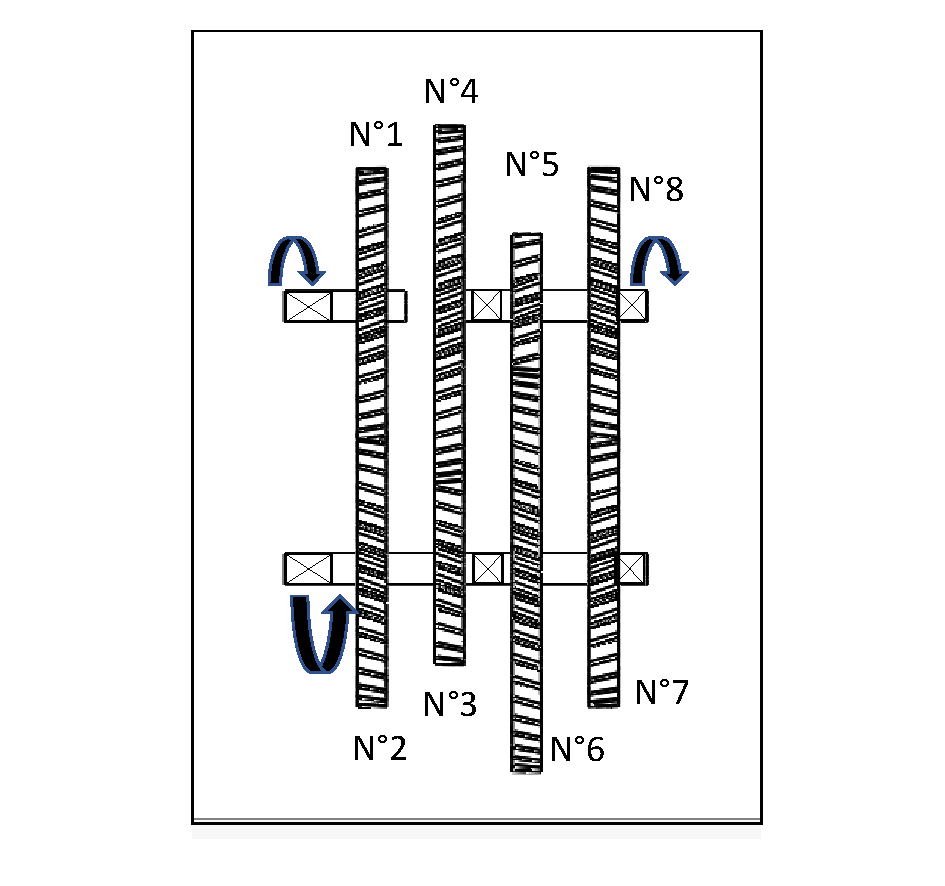
\includegraphics[width =0.5\textwidth, trim = {2cm, 0, 2cm, 0}]{Cap4_DisenoBasico/Figura/caja.pdf}
    \caption{Esquema básico del sistema de transmición}{Fuente: Elaboración propia}
    \label{fig:Transmición}
\end{figure}

\begin{table}[hbt]
    \centering
    \begin{tabular}{|c|c|}
        \hline
        \textbf{Dientes $N^{\circ}$} & \textbf{$N^{\circ}$ de dientes} \\ \hline
        1 & 34 \\ \hline
        2 & 34 \\ \hline
        3 & 51 \\ \hline
        4 & 17 \\ \hline
        5 & 45 \\ \hline
        6 & 23 \\ \hline
        7 & 34 \\ \hline
        8 & 34 \\ \hline
    \end{tabular}
    \caption{Número de dientes}
    \label{table:Transmición}
\end{table}


En la figura \ref{fig:Transmición}, se presenta un esquema de la caja de transmisión con el cual se trabajará a detalle posteriormente, esta cuenta con 8 engranajes y tres ejes, uno de entrada, uno de salida y uno intermedio. El número de dientes de cada engranaje se especifican en la tabla \ref{table:Transmición}.

\newpage
\newpage

%%%%%   Diseño Basico Mecanismo    %%%%%
\section{Diseño Básico del Mecanismo}
Para el diseño básico del mecanismo se trata en dos partes de análisis y dos partes de síntesis o dimensionamiento, esto ocurre porque se trata en dos niveles: el cinemático y el cinético. El primer nivel hace referencia a la parte de movimiento, sin tener en cuenta que lo produce. Por lo que en esta parte se eligen las dimensiones, conocidas como longitudes, que influyen el movimiento. El segundo nivel trata las causas del movimiento, analizando las fuerzas y/o torques necesarios para cumplir las trayectorias definidas.

Para el diseño básico de mecanismo se trabajará primero el nivel cinemático, con su respectivo análisis y dimensionamiento, para luego trabajar el nivel cinético, en donde se determinarán las relaciones para obtener las fuerzas de los actuadores, posterior a eso se plantea un diseño de rigidez que permita manejar los desplazamientos producidos durante la operación. Todo para que por medio de un método de optimización permite dimensionar el mecanismo para que no falle por desplazamiento.

\subsection{Análisis Cinemático}

\subsubsection{Definición de lazos de posición}
Para el mecanismo propuesto se plantean los lazos cinemáticos del sistema, teniendo como referencia el sistema coordenado en el centro de la base triangular, $O$ (Ver Figura \ref{fig:LazosVectoriales}). Por la simétrica del mecanismo, sus tres brazos presentan lazos vectoriales idénticos, por lo tanto, se puede describir el lazo de manera generalizada para el análisis.

Como se muestra en la Figura \ref{fig:LazosVectorialesArm}, la cadena cinemática presenta 6 puntos importantes. Estos puntos representan la ubicación de cada una de las juntas revolutas del dispositivo ($A$, $B$, $C$ y $D$), la ubicación del origen del sistema de referencia ($O$) y la ubicación de la herramienta de corte ($P$); en donde se interconectan la revoluta final de cada brazo.

Para el caso de  las revolutas $B$ y $D$ poseen su eje de giro normal al vector $\vec{CD}$, lo que producen el ángulo de elevación (en inglés \textit{pitch angle}) del brazo; además su ángulo, $\beta_i$ se mide con respecto al eje X local del eslabón $AB$ (ver Figura \ref{fig:LazosVectorialesABC}). Mientras que las revolutas $A$ y la ubicada en $P$ poseen su eje de giro a lo largo del eje Z, lo que simboliza el ángulo de giro (en inglés \textit{yaw angle}) del brazo; y su ángulo de posición, $\theta_i$, es relativo a la dirección del vector $\vec{OA}$ (ver Figura \ref{fig:LazosVectorialesTheta}). 

Las medidas del mecanismo son simbolizadas de la siguientes manera: la distancia entre los puntos $O$ y $A$ se simboliza con $R_{b}$ y se conoce como radio de la base; para la distancia entre $A$ y $B$ se representa con $L_A$; para el vector $\vec{BC}$ su magnitud se simboliza con $e$; para el vector $\vec{CD}$ la magnitud es $q_i$ y esta es la posición del actuador; por último, $PD$ es representado por $L_D$.

Referente al vector $\vec{OP}$ es representa la posición de la herramienta referente al sistema coordenado utilizando.

\begin{figure}[htb!]
    \centering
    \begin{subfigure}{0.6\textwidth}
        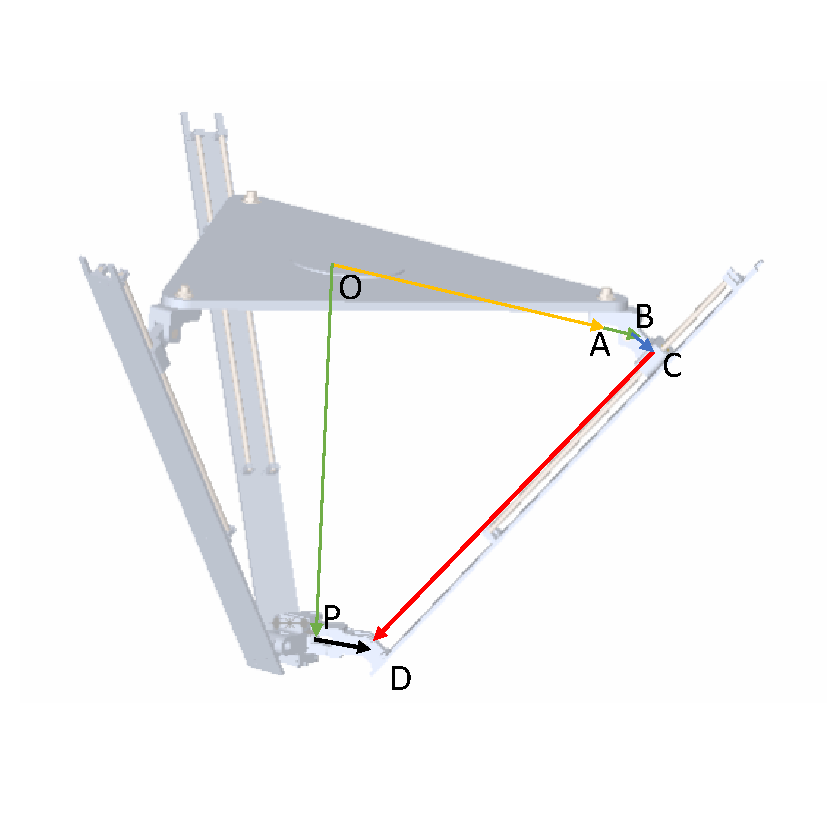
\includegraphics[width=0.9\linewidth]{Cap4_DisenoBasico/Figura/PDFLAZOS1.pdf}
        \caption{Lazos Vectoriales a lo largo de un brazo}
        \label{fig:LazosVectorialesArm}
    \end{subfigure}
    \begin{subfigure}{0.45\textwidth}
        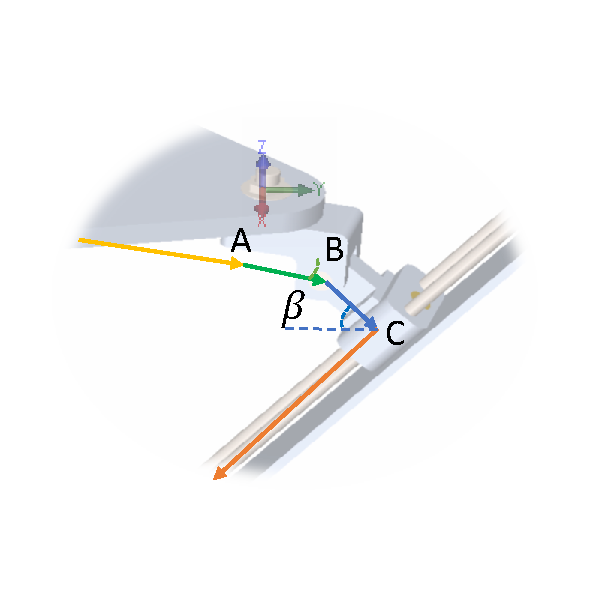
\includegraphics[width=0.9\linewidth]{Cap4_DisenoBasico/Figura/PDFLAZOS2.pdf}
        \caption{vista de detalle de los puntos ABC}
        \label{fig:LazosVectorialesABC}
    \end{subfigure}
    \begin{subfigure}{0.45\textwidth}
        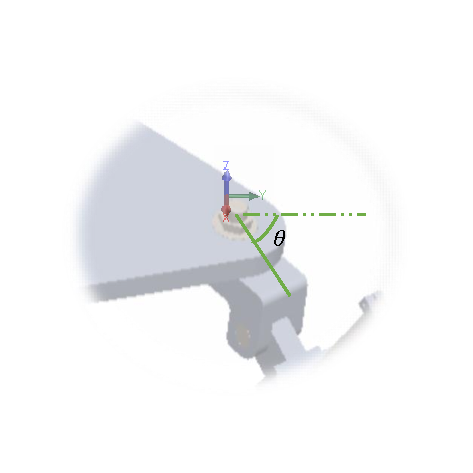
\includegraphics[width=0.9\linewidth]{Cap4_DisenoBasico/Figura/PDFLAZOS3.pdf}
        \caption{Posición angular de $ \theta $}
        \label{fig:LazosVectorialesTheta}
    \end{subfigure}
    \caption{Lazos Vectoriales del mecanismo}
    \label{fig:LazosVectoriales}
\end{figure}

La cadena cinemática queda de la forma:
\begin{equation}
    \vec{OA} + \vec{AB} + \vec{BC} + \vec{CD} = \vec{OP} + \vec{PD}
    \label{Eq:cadenacinematica}
\end{equation}

\subsubsection{Análisis de posiciones}
Para resolver el problema de posiciones del mecanismo, se hace uso de la ecuación cinemática establecida para un brazo general. Puesto que el efector final, $P$, del mecanismo tiene un movimiento lineal en espacio, su posición se representa con un vector de 3 coordenadas cartesianas cualquiera (ver Ecuación \ref{Eq:P}). Por otro lado,  los eslabones que son conectan por revolutas, se representa por la combinación de matrices de rotación (sección \ref{sec:FundamentosdelaRobotica}). 

\begin{equation}
    P = \left[\begin{array}{c} P_x \\ P_y \\ P_z \end{array} \right]
    \label{Eq:P}
\end{equation}

Con el fin de obtener las expresiones matemáticas generales para las posiciones, las variables de cada brazo manejan un subíndice $i$, el cual indica el brazo correspondiente por eso maneja los valores de $1, ~2, ~y~3$. Además de los parámetros dimensionales explicados en la sección anterior, es necesario la definición de $\alpha_i$, el ángulo que determina la posición de la revoluta $A$.

\begin{equation}
    \alpha_i = \frac{2\pi}{3}\left( i - 1 \right)
\end{equation}

Luego de esto, la primera expresión obtenida es la que asocia la posición del efector final, $P$, con el ángulo de giro $\theta_i$ de cada brazo:

\begin{equation}
    \theta _{i}=\arctan\left(\frac{P_{y}-R_{b}\,\sin\left(\alpha _{i}\right)}{P_{x}-R_{b}\,\cos\left(\alpha _{i}\right)}\right)-\alpha _{i}
\end{equation}

Ya obtenido el valor de $\theta_i$ es posible determinar $q_i$, sin embargo, para poderlo calcular es necesario determinar $M_i$ (ver ecuación \ref{Eq:M_i}):

\begin{subequations}
    \begin{eqnarray}
        q_{i}=\sqrt{M_i-e^2} \\
        \nonumber \\
        M_i =  \begin{array}{c}
            \left( R_b \cos\left(\alpha_i\right) + \left(L_A-L_D\right)\cos\left(\theta_i+\alpha_i\right) - P_x\right)^2 \\
            + \left( R_b \sin\left(\alpha_i\right) + \left(L_A-L_D\right)\sin\left(\theta_i+\alpha_i\right) - P_y\right)^2 \\
            + P_z^2 \label{Eq:M_i}
        \end{array}
    \end{eqnarray}
\end{subequations}

La última expresión obtenida es la que determina el valor de $\beta_i$, en donde se necesita de la tercera componente de $P$ y el valor de $q_i$:

\begin{equation}
    \beta_i = 2 \arctan\left( \frac{e+\sqrt{-{P_{z}}^2+e^2+{q_{i}}^2}}{P_{z}+q_{i}} \right)
\end{equation}

El desarrollo matematico para la obtención de estas expresiones mostrado en el anexo \ref{Anexo:AnalisisdePosiciones}.
\newpage

\subsubsection{Análisis de velocidades}
El análisis de velocidades comienza con la obtención del lazo de velocidades del brazo, para eso se deriva la cadena cinemática (Ecuación \ref{Eq:cadenacinematica}):

\begin{equation}
    \dot{\vec{AB}} + \dot{\vec{BC}} + \dot{\vec{CD}} = \dot{\vec{OP}} + \dot{\vec{PD}}
    \label{Eq:cadenavelocidades}
\end{equation}

Con esta nueva expresión aparecen incógnitas relacionadas con la velocidad de cambio de $\theta, q$ y $\beta$, además el sistema de ecuaciones que se genera es lineal por lo que se puede transformar en ecuaciones matriciales que modelen el comportamiento de la cada variable con respecto a la velocidad del punto $P$ (ver Ecuación \ref{Eq:dP}), y que estén de la siguiente forma:

\begin{equation}
    X = J_{X} \dot{P}
    \label{Eq:JacobianExample}
\end{equation}

\begin{equation}
    \dot{P} = \left[\begin{array}{c} \dot{P}_x \\ \dot{P}_y \\ \dot{P}_z \end{array} \right]
    \label{Eq:dP}
\end{equation}

En donde $ \dot{X} $ simboliza el vector con la incógnita para los 3 brazos, y $J_{X}$ es la matriz jacobiana que relaciona las velocidades del efector con la de las incógnitas, esto manejando la siguiente notación $C_X = \cos{\left( X \right)}$ y $S_X = \sin{\left( X \right)}$.

La primera matriz obtenida $J_{q}$, la cual determina las velocidades de los actuadores ($\dot{q}_{1}, \dot{q}_{2}, \dot{q}_{3}$): 

\begin{equation}
    J_{q} = \left[ \begin{array}{ccc}
        -C_{\alpha_1+\theta_1}C_{\beta_1} - \frac{eC_{\alpha_1+\theta_1}S_{\beta_1}}{q_1} & -S_{\alpha_1+\theta_1}C_{\beta_1} - \frac{eS_{\alpha_1+\theta_1}S_{\beta_1}}{q_1} & -S_{\beta_1} + \frac{eC_{\beta_1}}{q_1} \\
        -C_{\alpha_2+\theta_2}C_{\beta_2} - \frac{eC_{\alpha_2+\theta_2}S_{\beta_1}}{q_2} & -S_{\alpha_2+\theta_2}C_{\beta_2} - \frac{eS_{\alpha_2+\theta_2}S_{\beta_2}}{q_2} & -S_{\beta_2} + \frac{eC_{\beta_2}}{q_2} \\
        -C_{\alpha_3+\theta_3}C_{\beta_3} - \frac{eC_{\alpha_3+\theta_3}S_{\beta_3}}{q_3} & -S_{\alpha_3+\theta_3}C_{\beta_3} - \frac{eS_{\alpha_3+\theta_3}S_{\beta_3}}{q_3} & -S_{\beta_3} + \frac{eC_{\beta_3}}{q_3}
    \end{array} \right]
\end{equation}

La segunda obtenida, $J_{\theta}$, determina las velocidades de $\theta$ ($\dot{\theta}_{1}, \dot{\theta}_{2}, \dot{\theta}_{3}$): 

\begin{subequations}
    \begin{eqnarray}
        J_{\theta} = \left[ \begin{array}{ccc}
            S_{\alpha_1 + \theta_1}/k_1 & -C_{\alpha_1 + \theta_1}/k_1 & 0 \\
            S_{\alpha_2 + \theta_2}/k_2 & -C_{\alpha_2 + \theta_2}/k_2 & 0 \\
            S_{\alpha_3 + \theta_3}/k_3 & -C_{\alpha_3 + \theta_3}/k_3 & 0
        \end{array} \right] \\
        k_i = L_D - L_A + q_i C_{\beta_i} + eS_{\beta_i}
    \end{eqnarray}
\end{subequations}

La última obtenida, $J_{\beta}$, determina las velocidades de $\beta$ ($\dot{\beta}_{1}, \dot{\beta}_{2}, \dot{\beta}_{3}$): 

\begin{equation}
    J_{\beta} = \left[ \begin{array}{ccc}
        eC_{\alpha_1+\theta_1}S_{\beta_1}/q_1 & eS_{\alpha_1+\theta_1}S_{\beta_1}/q_1 & eC_{\beta_1}/q_1 \\
        eC_{\alpha_2+\theta_2}S_{\beta_2}/q_2 & eS_{\alpha_2+\theta_2}S_{\beta_2}/q_2 & eC_{\beta_1}/q_2 \\
        eC_{\alpha_3+\theta_3}S_{\beta_3}/q_3 & eS_{\alpha_3+\theta_3}S_{\beta_3}/q_3 & eC_{\beta_3}/q_3
    \end{array} \right]
\end{equation}
\newpage

\subsubsection{Análisis de aceleraciones}
El análisis de aceleraciones comienza con la obtención del lazo de aceleraciones del brazo, para eso se deriva la cadena de velocidades (Ecuación \ref{Eq:cadenavelocidades}.

\begin{equation}
    \ddot{\vec{AB}} + \ddot{\vec{BC}} + \ddot{\vec{CD}} = \ddot{\vec{OP}} + \ddot{\vec{PD}}
    \label{Eq:cadenaaceleraciones}
\end{equation}

A partir de eso se busca obtener expresiones para las aceleraciones de $\theta, q$ y $\beta$, conociendo la aceleración del efector (ver Ecuación \ref{Eq:ddP}). las cuales mantendrán la siguiente forma:

\begin{equation}
    \ddot{X} = J_{X} \ddot{P} + B_{X}
    \label{Eq:AcelerationExample}
\end{equation}

\begin{equation}
    \ddot{P} = \left[\begin{array}{c} \ddot{P}_x \\ \ddot{P}_y \\ \ddot{P}_z \end{array} \right]
    \label{Eq:ddP}
\end{equation}

En donde $J_{X}$ es el mismo jacobiano obtenido en velocidades, mientras que $B_{X}$ es un vector donde está contenido los efectos de las aceleraciones normales, así como la aceleración de coriolis experimentado por los brazos.

\begin{equation}
    B_{q} = \left[ \begin{array}{c}
        L_A\dot{\theta}_1^2\left(q_{1}C_{\beta_1} + eS_{\beta_1}\right)/q_{1}
        - e\left(2e\dot{\beta}_1^2 + e\dot{\theta}_1^2 - e\dot{\theta}_1^2C_{2\beta_1} + q_{1}\dot{\theta}_1^2S_{2\beta_1}\right)/2q_{1}^2 ~...\\
        ~~-\left(q_{1}\dot{\beta}_1^2 + q_{1}\dot{\theta}_1^2C_{\beta_1}^2 + 2e\dot{\beta}_1\dot{q}_1 + e\dot{\theta}_1^2S_{2\beta_1}/2\right) \\
        L_A\dot{\theta}_2^2\left(q_{2}C_{\beta_2} + eS_{\beta_2}\right)/q_{2}
        - e\left(2e\dot{\beta}_2^2 + e\dot{\theta}_2^2 - e\dot{\theta}_2^2C_{2\beta_2} + q_{2}\dot{\theta}_2^2S_{2\beta_2}\right)/2q_{2}^2 ~...\\
        ~~-\left(q_{2}\dot{\beta}_2^2 + q_{2}\dot{\theta}_2^2C_{\beta_2}^2 + 2e\dot{\beta}_2\dot{q}_2 + e\dot{\theta}_2^2S_{2\beta_2}/2\right) \\
        L_A\dot{\theta}_3^2\left(q_{3}C_{\beta_3} + eS_{\beta_3}\right)/q_{3}
        - e\left(2e\dot{\beta}_3^2 + e\dot{\theta}_3^2 - e\dot{\theta}_3^2C_{2\beta_3} + q_{3}\dot{\theta}_3^2S_{2\beta_3}\right)/2q_{3}^2 ~...\\
        ~~-\left(q_{3}\dot{\beta}_3^2 + q_{3}\dot{\theta}_3^2C_{\beta_3}^2 + 2e\dot{\beta}_3\dot{q}_3 + e\dot{\theta}_3^2S_{2\beta_3}/2\right)
    \end{array} \right]
\end{equation}

\begin{subequations}
    \begin{eqnarray}
        B_{\theta} = \left[ \begin{array}{c}
            \left( 2e\dot{\beta}_1\dot{\theta}_1C_{\beta_1} + 2\dot{\theta_1} \left( \dot{q}_1C_{\beta_1} - q_{1}\dot{\beta}_1S_{\beta_1}\right) \right)/k_1 \\
            \left( 2e\dot{\beta}_2\dot{\theta}_2C_{\beta_2} + 2\dot{\theta_2} \left( \dot{q}_2C_{\beta_2} - q_{2}\dot{\beta}_2S_{\beta_2}\right) \right)/k_2 \\
            \left( 2e\dot{\beta}_3\dot{\theta}_3C_{\beta_3} + 2\dot{\theta_3} \left( \dot{q}_3C_{\beta_3} - q_{3}\dot{\beta}_3S_{\beta_3}\right) \right)/k_3 \\
        \end{array} \right] \\
        k_i = L_D - L_A + q_i C_{\beta_i} + eS_{\beta_i}
    \end{eqnarray}
\end{subequations}

\begin{equation}
    B_{\beta} = \left[ \begin{array}{c}
        \left(-(L_A - L_D)\dot{\theta}_1^2S_{\beta_1} + e\left(\dot{\beta}_1^2 + \dot{\theta}_1^2S_{\beta_1}^2\right) + q_{1}S_{2\beta_1}\dot{\theta}_1^2/2 + 2\dot{\beta}_{1}\dot{q}_1\right)/q_{1} \\
        \left(-(L_A - L_D)\dot{\theta}_2^2S_{\beta_2} + e\left(\dot{\beta}_2^2 + \dot{\theta}_2^2S_{\beta_2}^2\right) + q_{2}S_{2\beta_2}\dot{\theta}_2^2/2 + 2\dot{\beta}_{2}\dot{q}_2\right)/q_{2} \\
        \left(-(L_A - L_D)\dot{\theta}_3^2S_{\beta_3} + e\left(\dot{\beta}_3^2 + \dot{\theta}_3^2S_{\beta_3}^2\right) + q_{3}S_{2\beta_3}\dot{\theta}_3^2/2 + 2\dot{\beta}_{3}\dot{q}_3\right)/q_{3}
    \end{array} \right]
\end{equation}

\newpage
\subsection{Comparativo con modelo SimMechanics}
Para la validación de las expresiones obtenidas en la sección anterior, se estableció un modelo en MATLAB/SIMULINK\textsuperscript{\textcopyright}, haciendo del paquete de simulación de múltiples cuerpos, SimMechanics. Para llevar a cabo esta comparación se dispusieron de las siguientes dimensiones: $R_b = 683.01~mm$, $L_A = 70.00~mm$, $L_D = 200.00~mm$ y $e = 57~mm$.

\begin{figure}[hb!]
    \centering
    \begin{subfigure}{0.9\textwidth}
        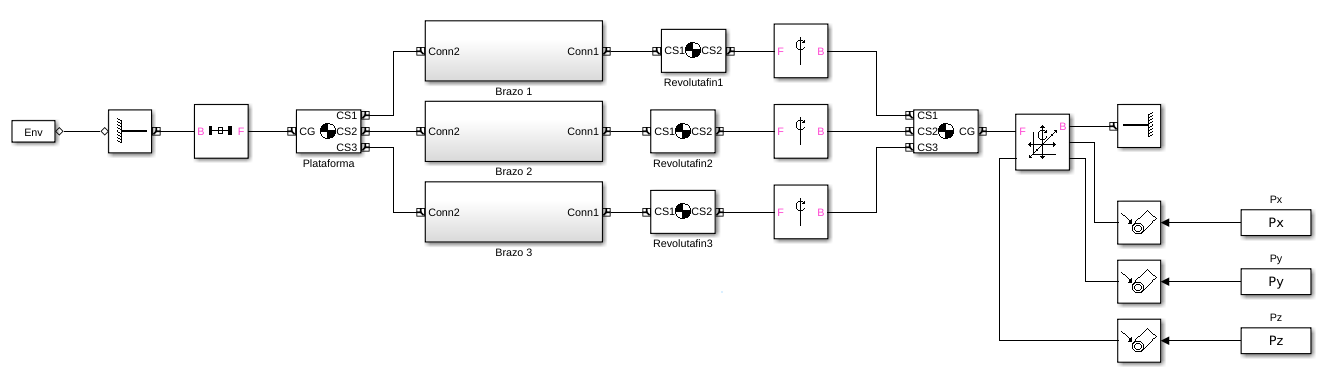
\includegraphics[width = \linewidth]{Cap4_DisenoBasico/Figura/ComparativoSimMechanics/EsquemaSimMechanicsGeneral.png}
        \caption{Esquema del Simulink General}
    \end{subfigure}
    \begin{subfigure}{0.9\textwidth}
        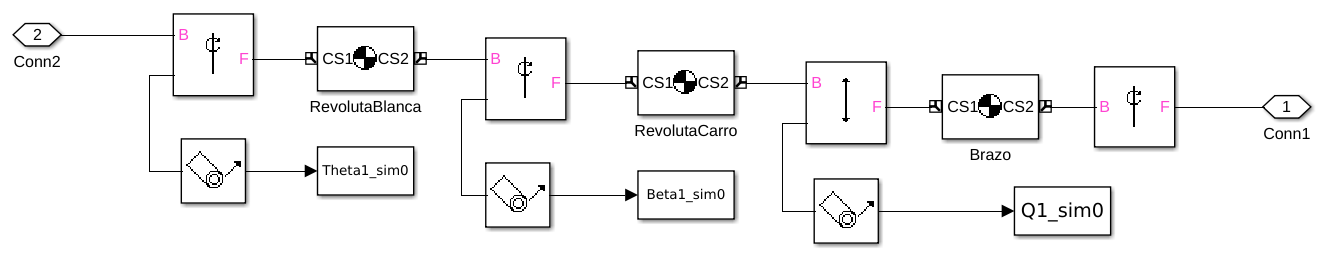
\includegraphics[width = \linewidth]{Cap4_DisenoBasico/Figura/ComparativoSimMechanics/EsquemaSimMechanicsArm.png}
        \caption{Esquema del Simulink Brazo}
    \end{subfigure}
    \begin{subfigure}{0.6\textwidth}
        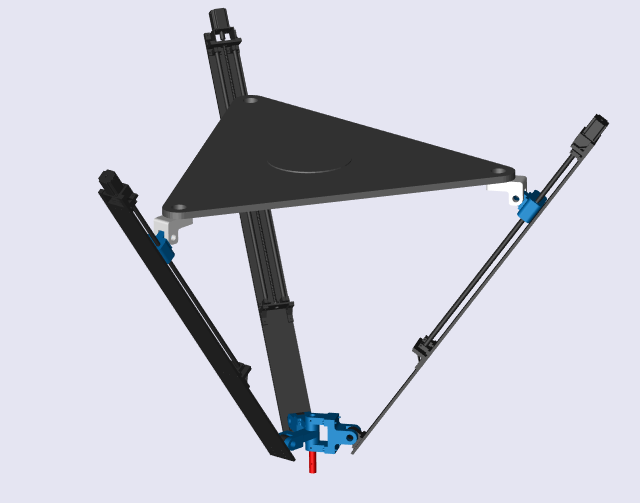
\includegraphics[width = \linewidth]{Cap4_DisenoBasico/Figura/ComparativoSimMechanics/ModelosSimMechanicsSolid.PNG}
        \caption{Visualización del SimMechanics}
    \end{subfigure}
    \caption{Esquema del modelo en SimMechanics}
\end{figure}

\begin{figure}
    \centering
    \begin{subfigure}{0.45\textwidth}
        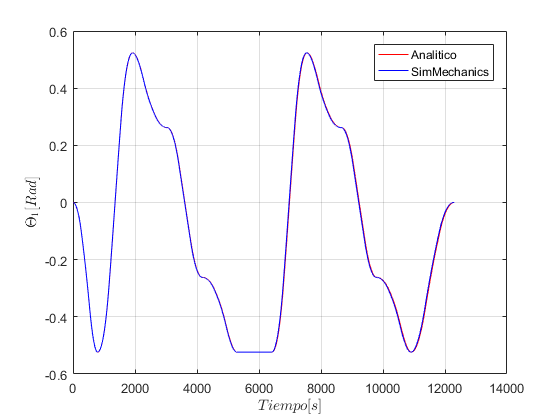
\includegraphics[width=\linewidth]{Cap4_DisenoBasico/Figura/ComparativoSimMechanics/Theta1.png}
        \caption{$\theta_1$}
    \end{subfigure}
    \begin{subfigure}{0.45\textwidth}
        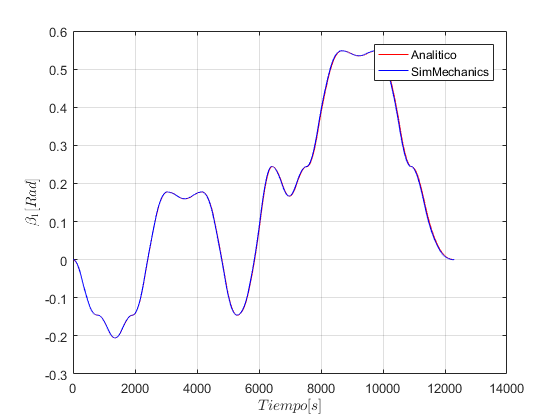
\includegraphics[width=\linewidth]{Cap4_DisenoBasico/Figura/ComparativoSimMechanics/Beta1.png}
        \caption{$\beta_1$}
    \end{subfigure}
    \begin{subfigure}{0.45\textwidth}
        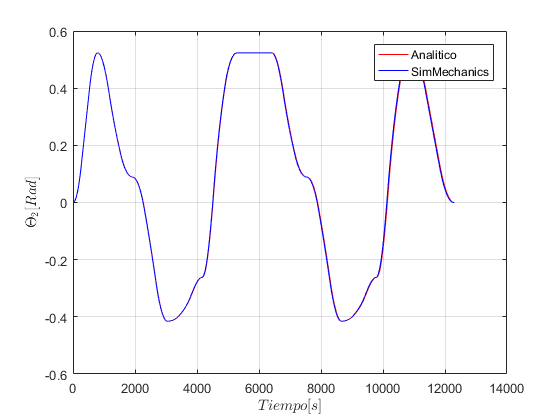
\includegraphics[width=\linewidth]{Cap4_DisenoBasico/Figura/ComparativoSimMechanics/Theta2.png}
        \caption{$\theta_2$}
    \end{subfigure}
    \begin{subfigure}{0.45\textwidth}
        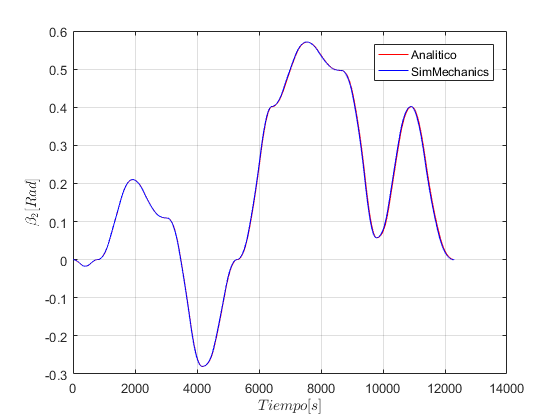
\includegraphics[width=\linewidth]{Cap4_DisenoBasico/Figura/ComparativoSimMechanics/Beta2.png}
        \caption{$\beta_2$}
    \end{subfigure}
    \begin{subfigure}{0.45\textwidth}
        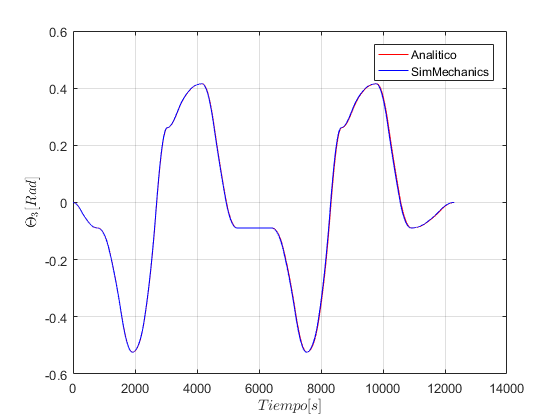
\includegraphics[width=\linewidth]{Cap4_DisenoBasico/Figura/ComparativoSimMechanics/Theta3.png}
        \caption{$\theta_3$}
    \end{subfigure}
    \begin{subfigure}{0.45\textwidth}
        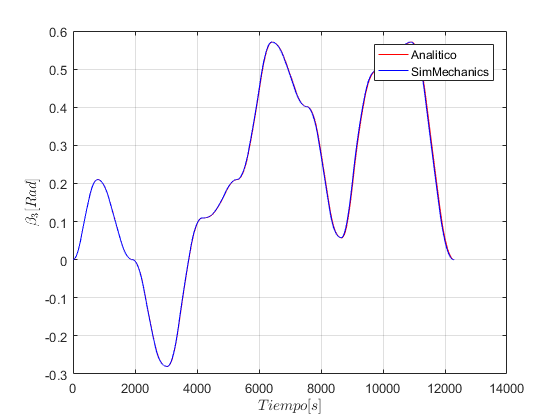
\includegraphics[width=\linewidth]{Cap4_DisenoBasico/Figura/ComparativoSimMechanics/Beta3.png}
        \caption{$\beta_3$}
    \end{subfigure}
    \caption{Comparación de posiciones de las revolutas $\theta$, $\beta$}
\end{figure}

\begin{figure}
    \centering
    \begin{subfigure}{0.45\textwidth}
        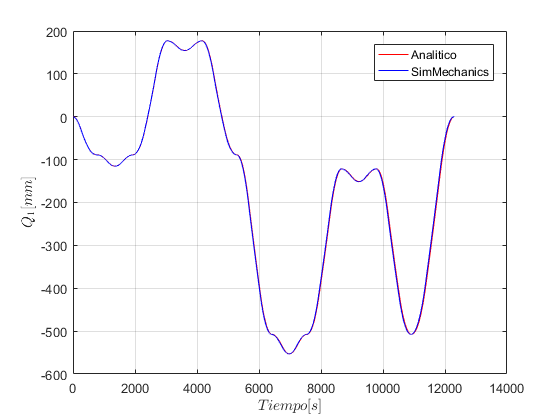
\includegraphics[width=\linewidth]{Cap4_DisenoBasico/Figura/ComparativoSimMechanics/Q1.png}
        \caption{$q_1$}
    \end{subfigure}
    \begin{subfigure}{0.45\textwidth}
        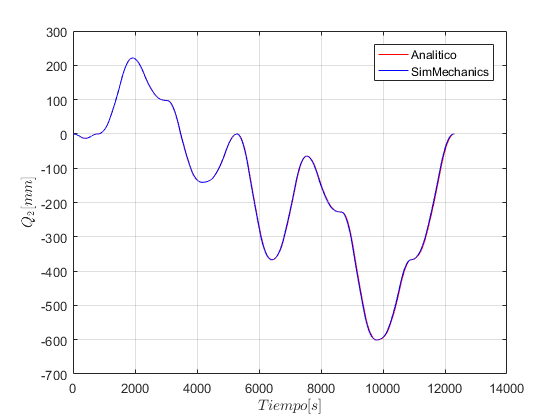
\includegraphics[width=\linewidth]{Cap4_DisenoBasico/Figura/ComparativoSimMechanics/Q2.png}
        \caption{$q_2$}
    \end{subfigure}
    \begin{subfigure}{0.45\textwidth}
        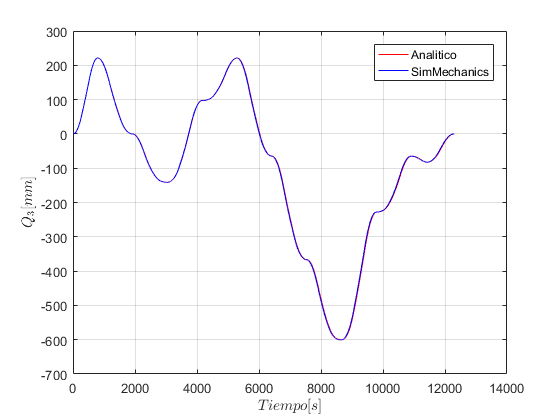
\includegraphics[width=\linewidth]{Cap4_DisenoBasico/Figura/ComparativoSimMechanics/Q3.png}
        \caption{$q_3$}
    \end{subfigure}
    \caption{Comparación de posiciones de los actuadores $q$}
\end{figure}

\begin{figure}
    \centering
    \begin{subfigure}{0.45\textwidth}
        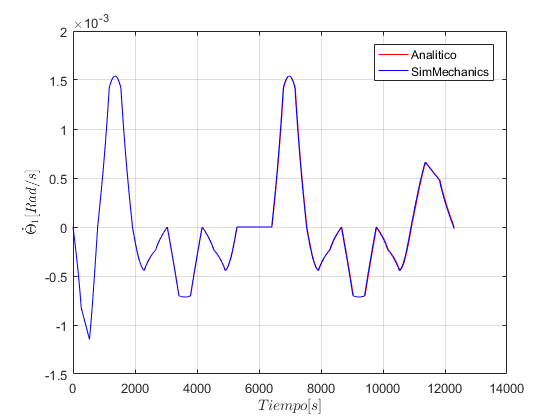
\includegraphics[width=\linewidth]{Cap4_DisenoBasico/Figura/ComparativoSimMechanics/Thetapunto1.png}
        \caption{$\dot{\theta}_1$}
    \end{subfigure}
    \begin{subfigure}{0.45\textwidth}
        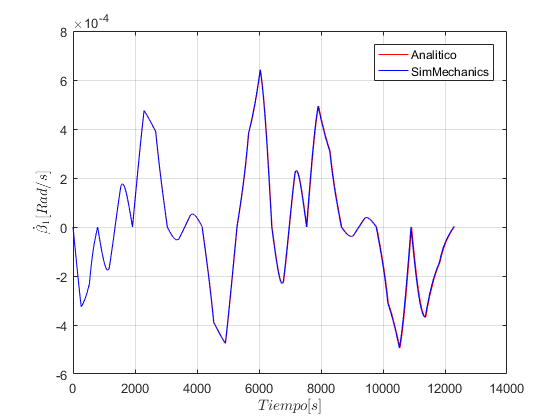
\includegraphics[width=\linewidth]{Cap4_DisenoBasico/Figura/ComparativoSimMechanics/betapunto1.png}
        \caption{$\dot{\beta}_1$}
    \end{subfigure}
    \begin{subfigure}{0.45\textwidth}
        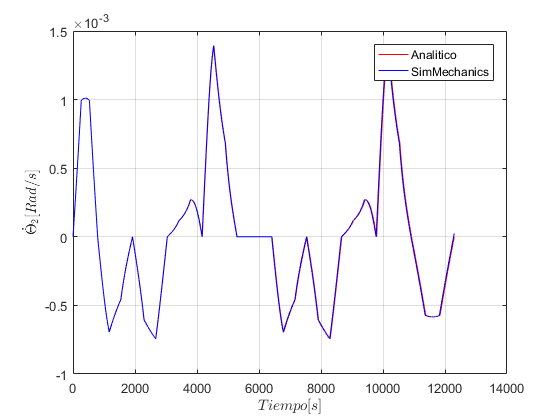
\includegraphics[width=\linewidth]{Cap4_DisenoBasico/Figura/ComparativoSimMechanics/Thetapunto2.png}
        \caption{$\dot{\theta}_2$}
    \end{subfigure}
    \begin{subfigure}{0.45\textwidth}
        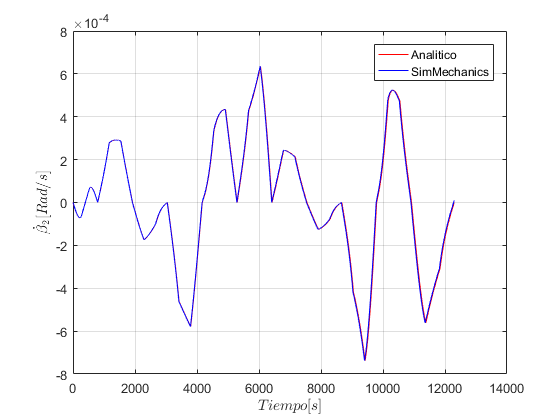
\includegraphics[width=\linewidth]{Cap4_DisenoBasico/Figura/ComparativoSimMechanics/betapunto2.png}
        \caption{$\dot{\beta}_2$}
    \end{subfigure}
    \begin{subfigure}{0.45\textwidth}
        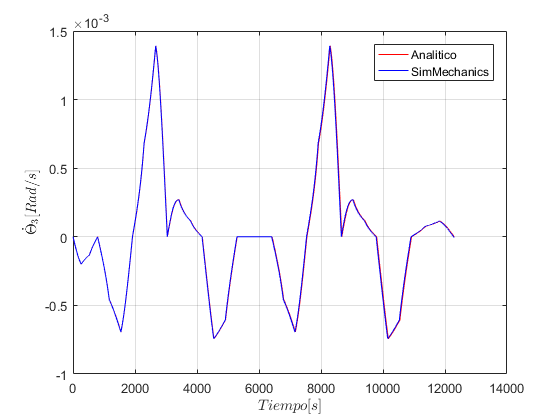
\includegraphics[width=\linewidth]{Cap4_DisenoBasico/Figura/ComparativoSimMechanics/Thetapunto3.png}
        \caption{$\dot{\theta}_3$}
    \end{subfigure}
    \begin{subfigure}{0.45\textwidth}
        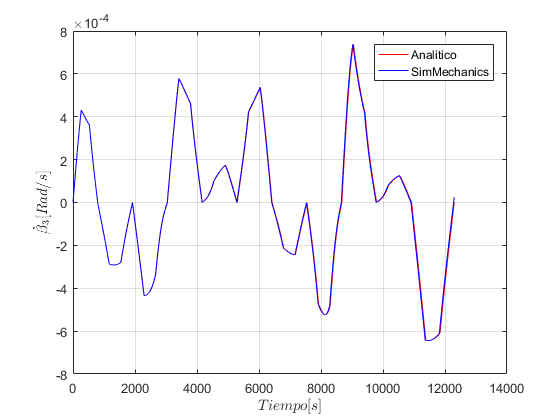
\includegraphics[width=\linewidth]{Cap4_DisenoBasico/Figura/ComparativoSimMechanics/betapunto3.png}
        \caption{$\dot{\beta}_3$}
    \end{subfigure}
    \caption{Comparación de velocidades de las revolutas $\dot{\theta}$, $\dot{\beta}$}
\end{figure}

\begin{figure}
    \centering
    \begin{subfigure}{0.45\textwidth}
        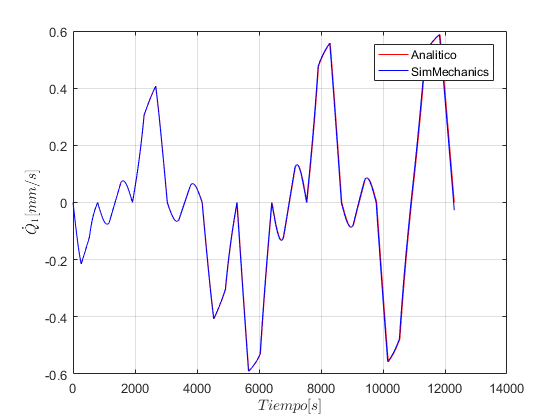
\includegraphics[width=\linewidth]{Cap4_DisenoBasico/Figura/ComparativoSimMechanics/Qpunto1.png}
        \caption{$\dot{q}_1$}
    \end{subfigure}
    \begin{subfigure}{0.45\textwidth}
        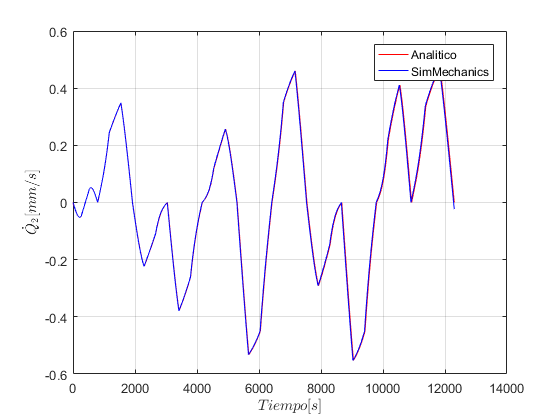
\includegraphics[width=\linewidth]{Cap4_DisenoBasico/Figura/ComparativoSimMechanics/Qpunto2.png}
        \caption{$\dot{q}_2$}
    \end{subfigure}
    \begin{subfigure}{0.45\textwidth}
        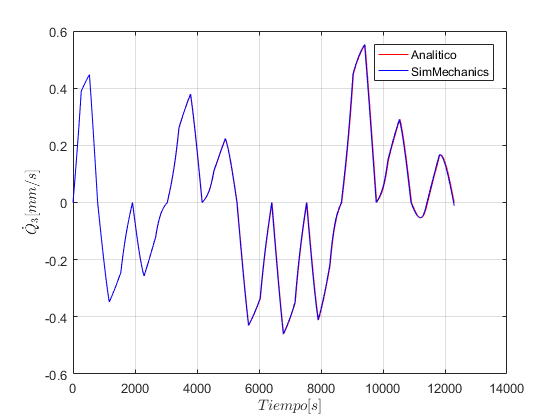
\includegraphics[width=\linewidth]{Cap4_DisenoBasico/Figura/ComparativoSimMechanics/Qpunto3.png}
        \caption{$\dot{q}_3$}
    \end{subfigure}
    \caption{Comparación de velocidades de los actuadores $\dot{q}$}
\end{figure}

\begin{figure}
    \centering
    \begin{subfigure}{0.45\textwidth}
        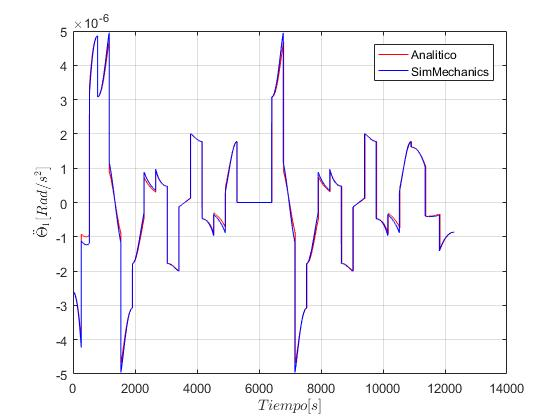
\includegraphics[width=\linewidth]{Cap4_DisenoBasico/Figura/ComparativoSimMechanics/ThetaPPunto1.jpg}
        \caption{$\ddot{\theta}_1$}
    \end{subfigure}
    \begin{subfigure}{0.45\textwidth}
        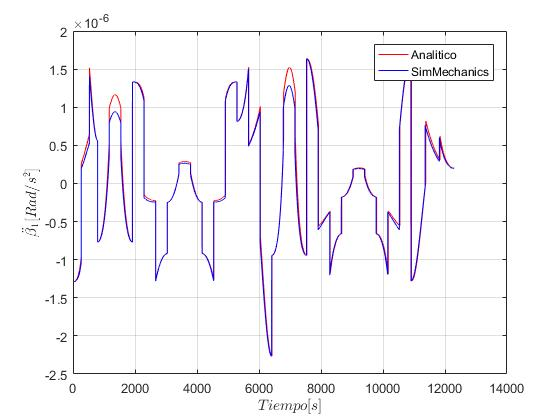
\includegraphics[width=\linewidth]{Cap4_DisenoBasico/Figura/ComparativoSimMechanics/BetaPPunto1.jpg}
        \caption{$\ddot{\beta}_1$}
    \end{subfigure}
    \begin{subfigure}{0.45\textwidth}
        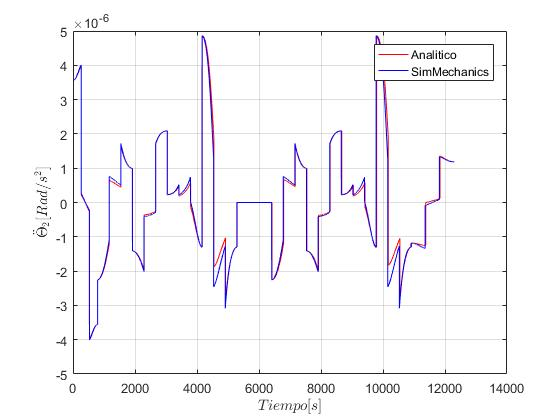
\includegraphics[width=\linewidth]{Cap4_DisenoBasico/Figura/ComparativoSimMechanics/ThetaPPunto2.jpg}
        \caption{$\ddot{\theta}_2$}
    \end{subfigure}
    \begin{subfigure}{0.45\textwidth}
        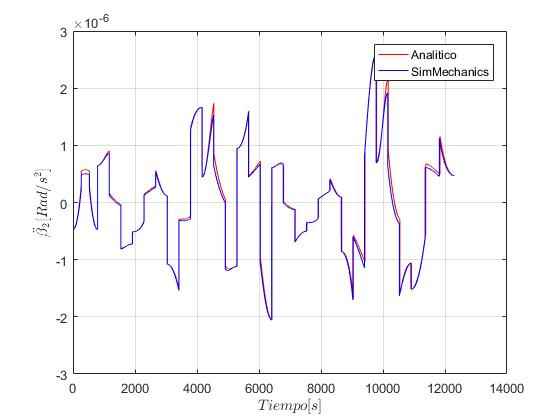
\includegraphics[width=\linewidth]{Cap4_DisenoBasico/Figura/ComparativoSimMechanics/BetaPPunto2.jpg}
        \caption{$\ddot{\beta}_2$}
    \end{subfigure}
    \begin{subfigure}{0.45\textwidth}
        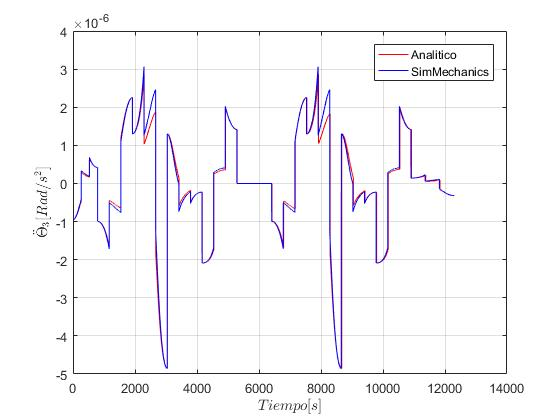
\includegraphics[width=\linewidth]{Cap4_DisenoBasico/Figura/ComparativoSimMechanics/ThetaPPunto3.jpg}
        \caption{$\ddot{\theta}_3$}
    \end{subfigure}
    \begin{subfigure}{0.45\textwidth}
        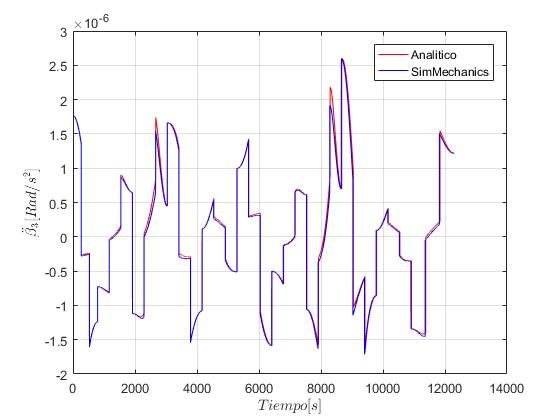
\includegraphics[width=\linewidth]{Cap4_DisenoBasico/Figura/ComparativoSimMechanics/BetaPPunto3.jpg}
        \caption{$\ddot{\beta}_3$}
    \end{subfigure}
    \caption{Comparación de aceleraciones de las revolutas $\ddot{\theta}$, $\ddot{\beta}$}
\end{figure}

\begin{figure}
    \centering
    \begin{subfigure}{0.45\textwidth}
        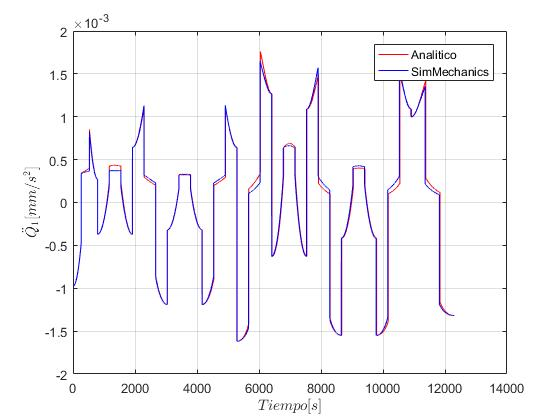
\includegraphics[width=\linewidth]{Cap4_DisenoBasico/Figura/ComparativoSimMechanics/QPPunto1.jpg}
        \caption{$\ddot{q}_1$}
    \end{subfigure}
    \begin{subfigure}{0.45\textwidth}
        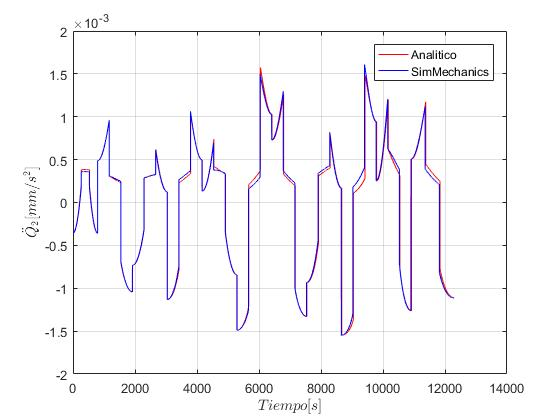
\includegraphics[width=\linewidth]{Cap4_DisenoBasico/Figura/ComparativoSimMechanics/QPPunto2.jpg}
        \caption{$\ddot{q}_2$}
    \end{subfigure}
    \begin{subfigure}{0.45\textwidth}
        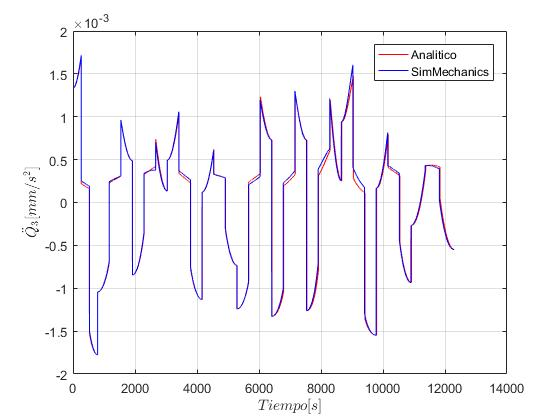
\includegraphics[width=\linewidth]{Cap4_DisenoBasico/Figura/ComparativoSimMechanics/QPPunto3.jpg}
        \caption{$\ddot{q}_3$}
    \end{subfigure}
    \caption{Comparación de aceleraciones de los actuadores $\ddot{q}$}
\end{figure}

\newpage
\subsection{Dimensionamiento Cinematico del Mecanismo}
En el diseño cinemático del mecanismo resulta de vital importancia un adecuado dimensionamiento de los elementos debido a el impacto que estos tienen en el desempeño del mismo. Esto lleva a buscar una manera de cuantificar y evaluar el desempeño cinemático de los robots por lo cual se propone utilizar alguno índices de desempeños propuestos en la literatura que relacionan las dimensiones y cinemática del mecanismo con el control, precisión, destreza e isotropía por todo el espacio de trabajo. 
Para la evaluación del desempeño cinemático del mecanismo se utiliza el Índice global de desempeño cinemático (Global Kinematic Performance Index) el cual está basado en la combinación de 4 índices de desempeño cinemático que son:

\textbf{Manipulabilidad}\newline
El índice de manipulabilidad brinda una medida de la capacidad general de posicionamiento y orientación de los actuadores sobre el efector final del mecanismo.
\begin{equation}
    M_{r}= \sqrt[m]{\lambda_1\lambda_2 ..\lambda_m}/l^2 
\end{equation}
$\lambda_i$ son los autovalores del jacobiano\newline
l es la suma de todas las longitudes de los elementos del mecanismo.\newline


\textbf{Velocidad Mínima}\newline
El índice de velocidad minima da un medida de la capacidad de respuesta del efector final en la dirección de menor rendimiento frente a cambios en los actuadores del sistema.
\begin{equation}
    V_{rmin}= \sqrt{min(\lambda_i)}/l
\end{equation}

\textbf{Isotropía de la Velocidad}\newline
El índice de isotropia mide la capacidad de transmisión de movimiento de manera uniforme en todas las direcciones y con un desempeño uniforme para ellas.
\begin{equation}
    \mu_{riso}= \sqrt[m]{\left(\frac{\sigma_1}{\sigma_{avg}}\right)\cdot\left(\frac{\sigma_2}{\sigma_{avg}}\right)...\left(\frac{\sigma_m}{\sigma_{avg}}\right)}
\end{equation}
$\sigma$ son los valores singulares del Jacobiano.\newline


\textbf{Precisión}\newline{}
El índice de precisión está relacionado con los errores de manufactura, errores de ensamblaje y errores en el control de posición. A medida que el índice aumenta la sensibilidad del mecanismo a estos errores es menor, es decir, presenta un mayor rendimiento.
\begin{equation}
    K_j = \frac{1}{||J||\cdot||J^+||}
\end{equation}

La evaluación de cada índice se realiza en todos los puntos del espacio de trabajo de manera discretizada, con los cuales se calcula un índice integral que considera diferentes aspectos de la distribucion del mismo.
\begin{equation}
    \xi_{integr} = (\alpha_1 \cdot\alpha_2\cdot \alpha_3 \cdot\alpha_4)(|\xi_{avg}| |\xi_{vol}| |\xi_{skew}| |\xi_{kurt}| )^T
\end{equation}
Donde:\newline
$\xi_{avg}$ es el valor promedio del índice $\xi$ en el espacio de trabajo. \newline
$\xi_{vol}$ es la volatilidad del índice en el espacio de trabajo. \newline
$\xi_{skew}$ es una medida de la asimetría de la distribución del índice. \newline
$\xi_{kurt}$ es el curtosis de la distribución del índice en el espacio de trabjo. \newline
$\alpha_i$ es el peso relativo de cada parámetro dentro del índice integral. \newline

El índice de desempeño global se calcula considerando los 4 índices calculados previamente
\begin{equation}
    \left(\textbf{GI}_{kine}\right)_{integr} = 
    \frac{\beta_1(M_r)_{integr}}{(M_r)_{norm}} +
    \frac{\beta_2(V_{rmin})_{integr}}{(V_{rmin})_{norm}} +
    \frac{\beta_3(\mu_{riso})_{integr}}{(\mu_{riso})_{norm}} +
    \frac{\beta_4(K_j)_{integr}}{(K_j)_{norm}} 
\end{equation}

Donde:\newline
$\beta_{i}$ es el peso de cada indice dentro del índice Global de Desempeño del mecanismo.\newline

% % % %    GA
En busca del mayor desempeño cinematico posible se desarrolló un algoritmo genetico con el fin de optimizar las dimensiones del mecanismo de forma tal que el Indice Global de Desempeño del robot sea el mayor posible. El algoritmo fue desarrollado en python y se presenta a continuación la rutina principal.

~
\begin{lstlisting}[frame=single,language = python]  % Start your code-block
import numpy as np
import matplotlib.pyplot as plt
import ga
import GlobalIndexKinematical as km

# Variables Range
span = [[500,50,50,-100],
        [1000,250,250,100]]

num_var = 4     #Numero de Variables a Optimizar
num_kromo = 10
pop_size = (num_kromo, 1)

new_pop1 = np.random.uniform(span[0][0], span[1][0], size=pop_size)
new_pop2 = np.random.uniform(span[0][1], span[1][1], size=pop_size)
new_pop3 = np.random.uniform(span[0][2], span[1][2], size=pop_size)
new_pop4 = np.random.uniform(span[0][3], span[1][3], size=pop_size)
new_population = np.concatenate((new_pop1,new_pop2, new_pop3,
                                new_pop4),axis=1)

# Point Cloud - WorkSpace
P = km.WorkspaceDesired(500.0,650.0,50.0)
num_parents = int(num_kromo/2) # Number of Parents
k = 120 # Number of Generations
Global_fitness, Avg_fitness, Mf_chromo=[],[],[]

for i in range(k):
    fitness = ga.fitnessK(new_population,P)
    Global_fitness.append(max(fitness))
    Avg_fitness.append(sum(fitness)/len(fitness))
    parents = ga.select_parents(new_population,fitness,num_parents)
    offspring_cross = ga.crossover(parents,num_kromo)
    mut_prob = 0.6
    offspring_mut = ga.mutation(offspring_cross,span, mut_prob)
    new_population = np.concatenate((parents, offspring_mut))

fitness = ga.fitnessK(new_population,P)
Global_fitness.append(max(fitness))
winner_chromo = new_population[fitness.index(max(fitness))]

win_local_idx = km.AllIndex(winner_chromo,P)
np.savetxt('win_local_idxs.csv', win_local_idx, delimiter = ',')
np.savetxt('Global_idx.csv',Global_fitness, delimiter = ',')
plt.plot(Global_fitness,'b-')
plt.plot(Avg_fitness,'r-')
plt.xlabel('# Generaciones')
plt.show()
\end{lstlisting}

El proceso de optimización con el algoritmo genético inicia con la generación de una poblacion aleatoria de cromosomas, es decir, generar un conjunto de soluciones posibles \textbf{new_population}. El siguiente paso es evaluar el desempeño de tal poblacion, para esto se considera el calculo del indice global de desempeño cinematico en los puntos discretizados \textbf{P} del espacio de trabajo. Para cada cromosoma de la población se obtienen los 4 indices descritos previamente, la integracion de estos y el valor del índice global.

\begin{lstlisting}[frame=single,language = python]  % Start your code-block

def fitnessK(population,P):
    fitness_population = []
    for L in population:
        I = km.AllIndex(L,P)
        I = km.IntegratedIndex(I)
        I = km.GlobalIndex(I).tolist()
        fitness_population.append(I[0][0])
    return fitness_population
\end{lstlisting}

A continuación se realiza la selección de los cromosomas más fuertes (aquellos con el desempeño más alto), los cuales sobreviviran y serán base para la generación siguiente.

\begin{lstlisting}[frame=single,language = python]  % Start your code-block

def select_parents(pop, fitness, num_parents):
    parents = np.zeros([num_parents,pop.shape[1]])
    for parent_num in range(num_parents):
        max_fit_index = np.where(fitness == np.max(fitness))
        max_fit_index = max_fit_index[0][0]
        parents[parent_num,:] = pop[max_fit_index,:]
        fitness[max_fit_index] = -999999999
    return parents
\end{lstlisting}







\newpage
\subsection{Análisis de Rigidez del Mecanismo}
Para el diseño de una herramienta CNC, la precisión es una de las especificaciones más importantes, debido a que esta determina la calidad de los productos, denotando un modo de falla distintivo para estos mecanismos. Puesto que la falta de precisión es producto de las deformaciones a las que está sometido el mecanismo, un método valido para analizar este factor en un mecanismo es el análisis de rigidez del sistema. Más específicamente, el método de elementos finitos, representando la rigidez del mecanismo por medio de matrices de rigidez; las cuales tienen en cuenta comportamientos elásticos y lineales dentro del sistema.

El elemento utilizado para la representación de los cuerpos es el Elemento de Marco Espacial (en inglés, Space Frame Element), por lo que es un elemento finito tridimensional con 12 grados de libertad. Esto es producto de sus dos nodos, los cuales poseen los 3 grados de libertad translaciones y rotacionales cada uno. Aparte de esto, el elemento de marco espacial conserva las siguientes propiedades constantes: Densidad $\rho$, Modulo de Elasticidad $E$, Modulo de Cortante Elástico $G$, Área transversal $A$, Momentos de Inercia de área $I_{y}$ y $I_{z}$, Momento Polar de Inercia $G$ y la longitud $L$.

\begin{figure}[hb!]
    \centering
    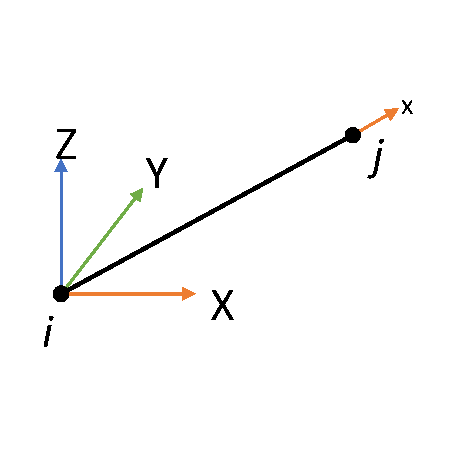
\includegraphics[width=0.30\textwidth]{Cap4_DisenoBasico/Figura/AnalisisRigidez/SPE.pdf}
    \caption{Elemento de Marco Espacial}
    \label{fig:SPE}
\end{figure}

La matriz de rigidez para este elemento es dada por la siguiente matriz:
\begin{equation}
    k = T^{T}k'T
\end{equation}

En donde $T$ es la matriz de rotación del sistema coordenado global al sistema local del elemento, la cual está conformada por $T_{i}$ que es una matriz $3\times3$ de cosenos directores, $T^T$ simboliza la transpuesta de esta matriz, $k$ es la matriz de rigidez del elemento en el sistema global mientras que $k’$ su versión en el sistema local. 

\begin{equation}
    T = \left[ \begin{array}{cccc}
        T_{i} & 0 & 0 & 0 \\
        0 & T_{i} & 0 & 0 \\
        0 & 0 & T_{i} & 0 \\
        0 & 0 & 0 & T_{i}
    \end{array} \right]
\end{equation}

\begin{footnotesize}
\begin{equation}
    k' = \left[\begin{array}{cccccccccccc} \frac{A\, E}{L} & 0 & 0 & 0 & 0 & 0 & -\frac{A\, E}{L} & 0 & 0 & 0 & 0 & 0\\ 0 & \frac{12\, E\, \mathrm{I_z}}{L^3} & 0 & 0 & 0 & \frac{6\, E\, \mathrm{I_z}}{L^2} & 0 & -\frac{12\, E\, \mathrm{I_z}}{L^3} & 0 & 0 & 0 & \frac{6\, E\, \mathrm{I_z}}{L^2}\\ 0 & 0 & \frac{12\, E\, \mathrm{I_y}}{L^3} & 0 & -\frac{6\, E\, \mathrm{I_y}}{L^2} & 0 & 0 & 0 & -\frac{12\, E\, \mathrm{I_y}}{L^3} & 0 & -\frac{6\, E\, \mathrm{I_y}}{L^2} & 0\\ 0 & 0 & 0 & \frac{G\, J}{L} & 0 & 0 & 0 & 0 & 0 & -\frac{G\, J}{L} & 0 & 0\\ 0 & 0 & -\frac{6\, E\, \mathrm{I_y}}{L^2} & 0 & \frac{4\, E\, \mathrm{I_y}}{L} & 0 & 0 & 0 & \frac{6\, E\, \mathrm{I_y}}{L^2} & 0 & \frac{2\, E\, \mathrm{I_y}}{L} & 0\\ 0 & \frac{6\, E\, \mathrm{I_z}}{L^2} & 0 & 0 & 0 & \frac{4\, E\, \mathrm{I_z}}{L} & 0 & -\frac{6\, E\, \mathrm{I_z}}{L^2} & 0 & 0 & 0 & \frac{2\, E\, \mathrm{I_z}}{L}\\ -\frac{A\, E}{L} & 0 & 0 & 0 & 0 & 0 & \frac{A\, E}{L} & 0 & 0 & 0 & 0 & 0\\ 0 & -\frac{12\, E\, \mathrm{I_z}}{L^3} & 0 & 0 & 0 & -\frac{6\, E\, \mathrm{I_z}}{L^2} & 0 & \frac{12\, E\, \mathrm{I_z}}{L^3} & 0 & 0 & 0 & -\frac{6\, E\, \mathrm{I_z}}{L^2}\\ 0 & 0 & -\frac{12\, E\, \mathrm{I_y}}{L^3} & 0 & \frac{6\, E\, \mathrm{I_y}}{L^2} & 0 & 0 & 0 & \frac{12\, E\, \mathrm{I_y}}{L^3} & 0 & \frac{6\, E\, \mathrm{I_y}}{L^2} & 0\\ 0 & 0 & 0 & -\frac{G\, J}{L} & 0 & 0 & 0 & 0 & 0 & \frac{G\, J}{L} & 0 & 0\\ 0 & 0 & -\frac{6\, E\, \mathrm{I_y}}{L^2} & 0 & \frac{2\, E\, \mathrm{I_y}}{L} & 0 & 0 & 0 & \frac{6\, E\, \mathrm{I_y}}{L^2} & 0 & \frac{4\, E\, \mathrm{I_y}}{L} & 0\\ 0 & \frac{6\, E\, \mathrm{I_z}}{L^2} & 0 & 0 & 0 & \frac{2\, E\, \mathrm{I_z}}{L} & 0 & -\frac{6\, E\, \mathrm{I_z}}{L^2} & 0 & 0 & 0 & \frac{4\, E\, \mathrm{I_z}}{L} \end{array}\right]
\end{equation}
\end{footnotesize}

Por consecuencia de la definición del elemento de marco espacial, una estructura con $n$ nodos, la matriz de rigidez de la estructura, $K$, será de $6n\times6n$. Además, para ensamblar la matriz de rigidez global es necesario sumar la submatrices de rigidez de cada elemento en sus respectivos espacios, esto al final genera la siguiente ecuación:

\begin{equation}
    \vec{F} = K \vec{U}
\end{equation}

Donde $\vec{U}$ es un vector que contiene los desplazamientos globales, tanto translaciones como angulares, de todos los nodos y $\vec{F}$ son las fuerzas y momentos globales aplicadas en cada nodo.

Para el modelo del mecanismo en elementos finitos se hicieron dos modificaciones, con el facilitar el modelamiento del mismo (Ver Figura \ref{fig:MecanismoDiscretizado}). La primera modificación fue realizada en la base, que se transformó de una placa triangular con los vértices redondeados a una serie de tubos de rectangular que cumplan la disposición geométrica de la placa forma. La segunda modificación fue eliminar el sistema paralelo de dos ejes sobre el perfil, a solo haber un eje en paralelo con el perfil. Cabe resaltar que el sistema de accionamiento no fue considerado para este análisis.El procedimiento utilizado para el modelo fue obtenido de \cite{kattan2010matlab}.

\begin{figure}[hbt!]
    \centering
    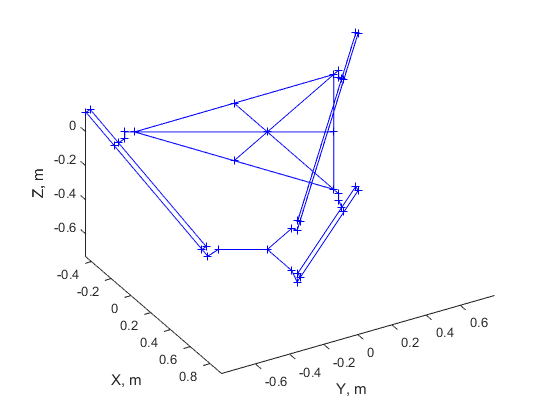
\includegraphics[width=\textwidth]{Cap4_DisenoBasico/Figura/AnalisisRigidez/MecanismoDiscretizado.png}
    \caption{Esquema de la discretización del mecanismo}
    \label{fig:MecanismoDiscretizado}
\end{figure}
\newpage

El modelo manejo dos tipos de material, más específicamente el acero y el aluminio, esto con el objetivo de obtener pesos ligeros en los materiales que no presentan deformaciones significativas y resistencia en aquellos elementos críticos. Los valores utilizados para la simulación son los siguientes:

\begin{longtable}{|c|c|c|c|}
    \hline \rowcolor[gray]{0.85}
    \textbf{Material} & \textbf{Densidad} & \textbf{Modulo de Elasticidad} & \textbf{Modulo de Cortante} \\ \rowcolor[gray]{0.85}
     & $\rho$ [$kg/m^3$] & $E$ [$GPa$] & $G$ [$GPa$] \\ \hline
     Acero & $7850.00$ & $200.00$ & $79.3$ \\ \hline
     Aluminio & $2700.00$ & $69.00$ & $27.00$ \\ \hline
     \caption{Lista de Materiales para el análisis de rigidez}
\end{longtable}

A partir de la discretización del mecanismo (ver Figura \ref{fig:MecanismoDiscretizado}) se establecieron 38 nodos distribuidos en 48 elementos que siguen la siguiente configuración:

\begin{longtable}{|c|c|c|c|c|}
    \hline \rowcolor[gray]{0.85}
    \textbf{Elemento} & \textbf{Material} & \textbf{Perfil Transversal} & \textbf{Componente} & \textbf{Dimensiones} \\ \hline \endhead
     1 : 12 & Acero     & Tuberia Rectangular \Rectpipe & Base          & $B, H, t$ \\ \hline %1
    13 : 15 & Aluminio  & Rectangular $\blacksquare$    & Revoluta AB   & $B, H$ \\ \hline %2
    16 : 18 & Aluminio  & Rectangular $\blacksquare$    & Revoluta AB   & $B, H$ \\ \hline %3
    19 : 21 & Aluminio  & Rectangular $\blacksquare$    & Revoluta BC   & $B, H$ \\ \hline %4
    22 : 24 & Acero     & Circular $\bullet$            & Eje del Brazo & $D$ \\ \hline %5
    25 : 27 & Aluminio  & Rectangular $\blacksquare$    &Soporte del Eje& $B, H$ \\ \hline %6
    28 : 33 & Aluminio  & Viga en T \Tsteel             & Brazo         & $B, H, t$ \\ \hline %7
    34 : 36 & Aluminio  & Rectangular $\blacksquare$    & Revoluta D    & $B, H$ \\ \hline %8
    37 : 39 & Aluminio  & Rectangular $\blacksquare$    & Revoluta DP   & $B, H$ \\ \hline %9
    40 : 42 & Aluminio  & Viga en T \Tsteel             & Brazo         & $B, H, t$ \\ \hline %10
    43 : 45 & Aluminio  & Rectangular $\blacksquare$    &Soporte del Eje& $B, H$ \\ \hline %11
    46 : 48 & Acero     & Rectangular $\blacksquare$    & Eje del Brazo & $B, H$ \\ \hline %12
    \caption{Configuraciones de los elementos}
\end{longtable}

Posterior a esto, las condiciones de frontera utilizadas para resolver este sistema son los nodos $3$, $5$ y $7$ son nodos fijos, es decir, para el análisis no presentan ningún tipo de desplazamiento o empotrados. Además, por las condiciones normales de operación se pueden despreciar los efectos de las aceleraciones dentro del sistema; quedando fuerzas externas al mecanismo, las fuerzas de corte y los pesos de los mismos elementos.

\newpage
\subsection{Dimensionamiento Cinético del Mecanismo}
Para el dimensionamiento cinético del mecanismo aplicado para las operaciones de maquinado se deben seguir diseñar contra los modos de falla más críticos de la operación. Para este caso el diseño básico se centró en la falla por deformación excesiva, la cual causa una pérdida de la precisión y seguimiento a la trayectoria por parte del dispositivo. Con este fin se dispuso del análisis de rigidez, sirviendo de herramienta matemática la obtención del resto de las dimensiones del mecanismo. Esto recordando que las longitudes fueron determinadas en el diseño cinemático, siendo estas $R_b = 675~mm, L_A = 50~mm, L_D = 249~mm$ y $e = 0~mm$.

El dimensionamiento fue realizado por un método iterativo se suponían unas dimensiones de las secciones transversales de los distintos elementos, observando la distribución de los desplazamientos que podía alcanzar el efector final a lo largo del espacio de trabajo. además se supuso que las fuerzas de corte estaba alineadas en el eje X y con un valor de $1.5~kN$.

\begin{longtable}{|c|c|c|c|c|}
    \hline
    \rowcolor[gray]{0.85}
     &  &  & \textbf{Parámetros} & \textbf{Parámetros} \\
    \rowcolor[gray]{0.85} \textbf{Componente} & \textbf{Perfil Transversal} & \textbf{Dimensiones} & \textbf{iniciales} & \textbf{finales} \\
    \rowcolor[gray]{0.85} & & & mm & mm \\\hline
    Base
         & Tuberia Rectangular \Rectpipe & $H,B,t$ & $70,40,5$ & $50,150,10$ \\ \hline
    \multirow{2}{*}{Revoluta AB}
         & Rectangular $\blacksquare$ & $H,B$ & $80,45$ & $80,45$ \\
         & Rectangular $\blacksquare$ & $H,B$ & $20,80$ & $20,80$ \\ \hline
    RevolutaBC
         & Rectangular $\blacksquare$ & $H,B$ & $45,45$ & $30,45$ \\ \hline
    Eje del Brazo
         & Circular $\bullet$         & $D$   & $16$    & $25.4$  \\ \hline
    Soporte del Eje
         & Rectangular $\blacksquare$ & $H,B$ & $45,45$ & $45,45$ \\ \hline
    Brazo
         & Viga en T \Tsteel          &$H,B,t$& $150,100,10$ & $150,100,15$ \\ \hline
    Revoluta D
         & Rectangular $\blacksquare$ & $H,B$ & $60,60$ & $70,70$ \\ \hline
    Revoluta DP
         & Rectangular $\blacksquare$ & $H,B$ & $60,60$ & $50,70$ \\ \hline
    \caption{Parámetros iniciales y finales para probar el mecanismo}
\end{longtable}

Luego de establecer los parámetros, prosiguió a evaluar bajo las condiciones de operación los desplazamientos alcanzados por el efector a lo largo del espacio de trabajo discretizado en una nube de puntos. Generando el siguiente histograma, ver Figura \ref{fig:Comparacion}, en donde se puede observar la distribución de los desplazamientos de $P$, mostrando que los parámetros iniciales presenta una alta variabilidad a lo largo del espacio de trabajo mientras que los parámetros finales presenta una baja variabilidad y un promedio mucho más bajo que el de los iniciales.


\newpage
